\documentclass[titlepage]{report}
\usepackage[italian]{babel}
\usepackage[babel]{csquotes}
\usepackage[a4paper,left=2cm,bottom=2cm,right=2cm,top=2.5cm]{geometry}
\usepackage[style=numeric-comp,useprefix,hyperref,backend=bibtex,natbib,sorting=none]{biblatex}
\usepackage{subcaption}
\usepackage{url}
\usepackage{graphicx} 			% pacchetto per inserire immagini
\usepackage{sidecap}			% pacchetto delle didascalie laterali
\usepackage{setspace}			% pacchetto per modificare interlinea
\usepackage{textcomp} 			% pacchetto per simboli unicode
\usepackage[table]{xcolor}		% pacchetto colori per le celle delle tabelle
\usepackage{float}
\usepackage{hyperref}
\usepackage{fancyhdr}
\usepackage[nowrite,infront,standard,swapnames]{frontespizio}

\begin{document}
	
\hypersetup{
	linkbordercolor={1 1 1},
}

\begin{frontespizio}
	\Universita {Brescia}
	\Logo [3cm]{Logo_unibs.pdf}
	\Dipartimento {Ingengeria dell'Informazione}
	\Corso [Laurea magistrale]{Ingegneria Elettronica}
	\Annoaccademico {2020--2021}
	\Titoletto{Progetto di Sistemi Elettronici Analogici}
	\Titolo {Circuito per la generazione del tono \\ (sinusoidale a frequenza variabile) per Theremin}
	\Sottotitolo{Progetto n°17}
	\NCandidati{Autori}
	\Candidato [706005]{Luca Brescia}
	\Candidato [89521]{Simone Pezzottini}
\end{frontespizio}
	
\tableofcontents

\chapter*{Obiettivo}
	\label{ch:Scope}
	\addcontentsline{toc}{chapter}{Obiettivo}
	\large Realizzazione di un tono a frequenza variabile nello spettro delle frequenze udibili [$20Hz - 20kHz$] utilizzando un VCO e una capacità variabile con il movimento di una mano seguendo lo schema a blocchi mostrato in \textit{Figura \ref{fig:Schema_Assegnazione}}. Il segnale modulato avrà un range di frequenze elevato, di conseguenza andrà mixato ad una sinusoide a frequenza determinata, per riportare lo spettro del segnale nel range delle frequenze udibili, e opportunamente filtrato per eliminare le componenti indesiderate.
	\\
	\\
	\begin{figure}[h]
		\centering
		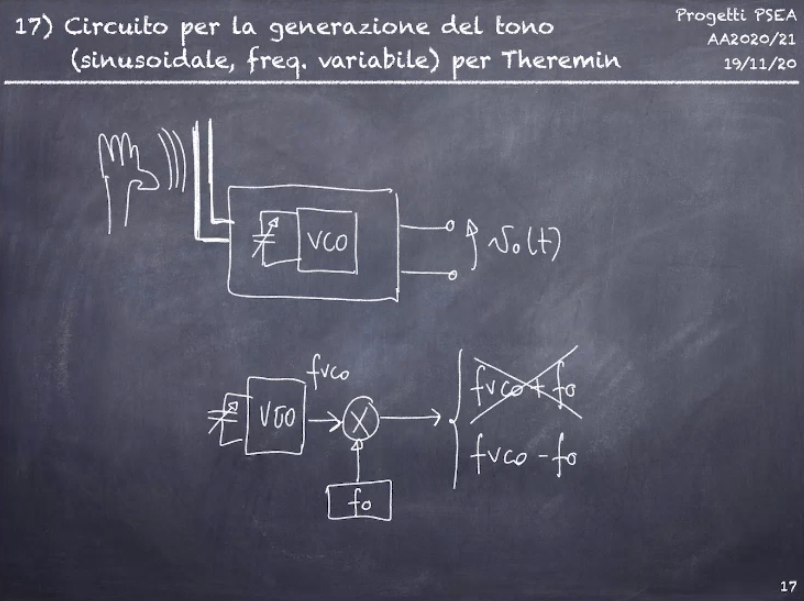
\includegraphics[scale=0.5]{Immagini/Schema_progetto_17.png}
		\caption{Schema generale di funzionamento di un circuito per la realizzazione di un tono.}
		\label{fig:Schema_Assegnazione}
	\end{figure}

	 In generale lo schema richiesto per la realizzazione del progetto potrebbe essere il seguente:
	 
	\begin{figure}[htbp]
		\centering
		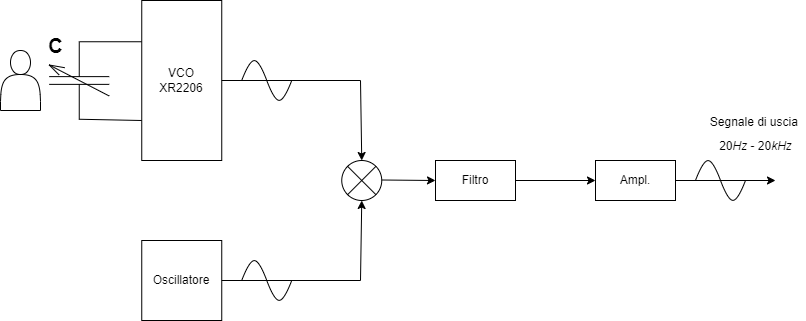
\includegraphics[scale=0.5]{Immagini/Schema Generale PSEA.png}
		\caption{Schema a blocchi generale del progetto}
		\label{fig: schema a blocchi generico}
	\end{figure}	


\newpage

	
\chapter{Scelta dei componenti}
	\label{ch:Scelta_componenti}
	I blocchi minimi necessari alla realizzazione di questo progetto sono:
	
	\begin{enumerate}
		\item Oscillatore sinusoidale a frequenza variabile(controllato in tensione (\textit{VCO}));
		\item Moltiplicatore analogico;
		\item Oscillatore a frequenza fissata;
		\item Filtro passa basso.
		\item Filtro passa alto con Amplificazione
	\end{enumerate}
	
	\noindent La scelta dei componenti è stata fatta considerando le caratteristiche del segnale da generare. In particolare, volendo realizzare uno shift in frequenza, pertanto vi è la necessità di lavorare con integrati con una banda passante adeguata.
	Avendo a disposizione una serie limitata di componenti si è deciso di utilizzare i seguenti:
	
	\begin{enumerate}
		\item per l'ossillatore a frequenza variabile si è scelto l'oscillatore monolitico \textit{XR2206} come \textit{VCO};
		\item Il moltiplicatore analogico \textit{AD633} per lo shift frequenziale;
		\item L'amplificatore operazionale \textit{LF353N} per la realizzazione dell oscillatore a ponte di Wien per la generazione della sinusoide di riferimento;
		\item L'amplificatore \textit{LF356P} per la realizzazione di filtro passa basso.
		\item L'amplificatore \textit{UA741} per la realizzazione dei filtri passa alto.
	\end{enumerate}
	
	
\section{Amplificatori operazionali LF353N, LF356P e uA741}
\label{sec:OpAmp}
	La scelta di questi componenti tra quelli disponibili è stata fatta principalmente per le bande bassanti dei dispositivi.
	\\ Sono necessari componenti a banda elevata poiché, come risulta dal capitolo \ref{ch:Risultati}, si deve lavorare con frequenze dell'ordine delle centinaia di kHz.
	
	 \noindent Infatti le bande in gioco sono di circa \textit{3MHz} per \textit{LF356P} mentre \textit{5MHz} per \textit{LF353N}. Ad esempio, l'\textit{UA741} ha un \textit{GBP} di \textit{1MHz} tipico. I primi due operazionali sono stati scelti per:
	
	\begin{enumerate}
		\item \textit{LF356N} per l'oscillatore armonica fondamentale 
		\item \textit{LF353P} per il filtro passa basso del 4o ordine. 
	\end{enumerate}
	
	
	\noindent Importante osservare che l'\textit{LF356P} ha al suo interno due amplificatori operazionali per cui è stato scelto per la realizzazione del filtro del $4^{o}$ ordine in modo da ridurre il numero di integrati per la realizzazione del dispositivo.Inoltre, l'\textit{LF353N}, avente una \textit{GBP} maggiore (\textit{5MHz}), permette di generare sinusoidi con un range di frequenze maggiore; altro motivo per cui si sono scelti i componenti come spiegato sopra.
	L'\textit{UA741} viene impiegato come filtro attivo passa alto del primo ordine $(e come amplificatore finale)$ per togliere le componenti inferiori a 20Hz come richiesto dal progetto e sfruttare contemporaneamente la banda passante ridotta del dispositvo al fine di attenuare le alte frequenze indesiderate.

	\noindent I motivi per cui le frequenze in gioco risultino essere elevate sono indicate nel capitolo \ref{ch:Risultati}.

	


	\begin{figure}[H]
		\centering
		\subfloat[][\emph{uA741}]
		{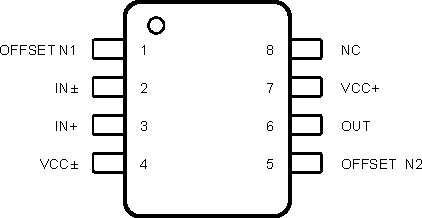
\includegraphics[width=.40\textwidth]{Immagini/ua741_pinout.pdf}} \qquad
		\subfloat[][\emph{LF353N}]
		{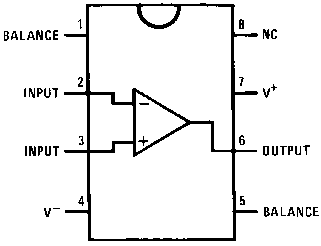
\includegraphics[width=.30\textwidth]{Immagini/lf353n_pinout.pdf}} \qquad 
		\subfloat[][\emph{LF356P}]
		{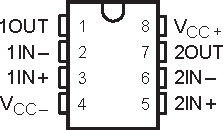
\includegraphics[width=.40\textwidth]{Immagini/lf356p_pinout.pdf}} \\
		\caption{PinOut dei tre Amplificatori Operazionali usati}
		\label{fig:pinout_OpAmp}
	\end{figure}

	
\section{Oscillatore monolitico XR2206}
	\label{sec:XR2206}
	
	Si è scelto di utilizzare \textit{XR2206} perché permette la generazione di diverse forme d'onda sinusoidali, onde quadre, rampe, onde triangolari ed impulsi garantendo un'alta precisione, stabilità e una bassa distorsione. L'ampiezza e la frequenza dei segnali in uscita sono direttamente modulabili dall'integrato, gestendo opportunamente gli ingressi. La gamma di frequenze generabili va da 0.01 $Hz$ a 1 $MHz$, quindi perfetto per le specifiche richieste dal progetto. 
	In \textit{Figura \ref{fig:sch_xr2206}} è mostrato lo schema a blocchi del componente.
	
	\begin{figure}[H]
		\centering
		\subfloat[][\emph{Schema dei collegamenti interni}]
		{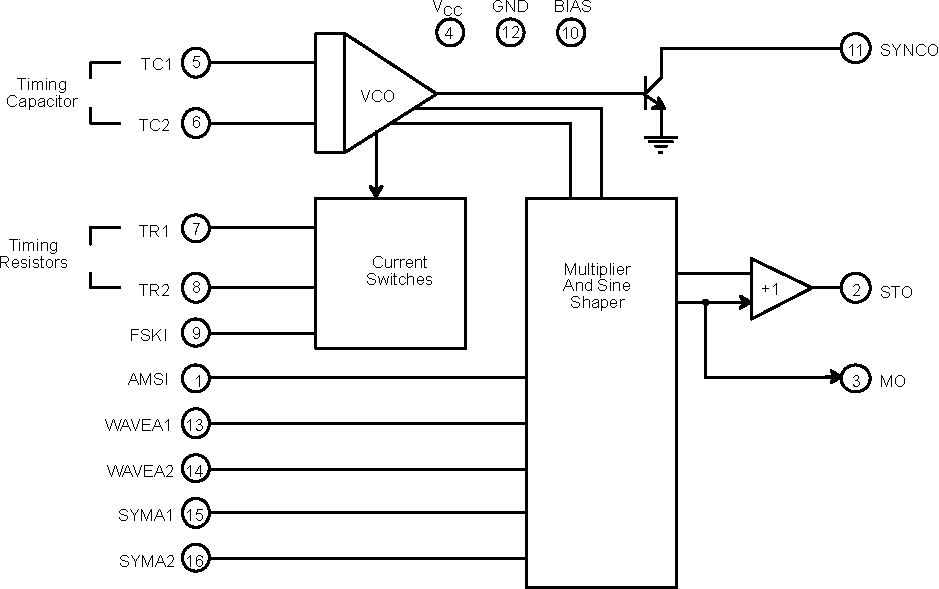
\includegraphics[width=.40\textwidth]{Immagini/schema_blocchi_xr2206.pdf}} \qquad
		\subfloat[][\emph{Descrizione in dettaglio dei pin}]
		{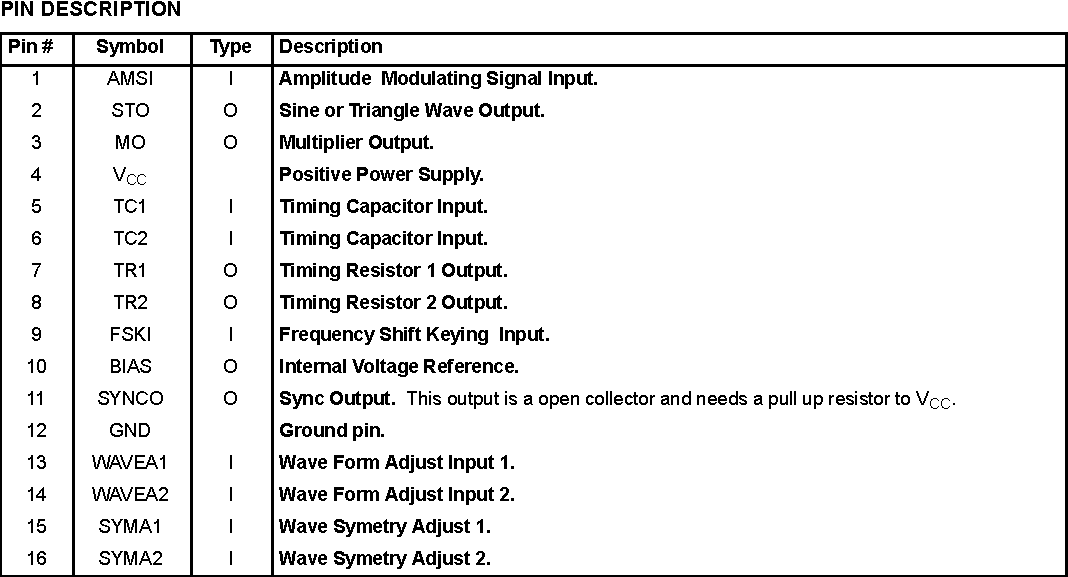
\includegraphics[width=.5\textwidth]{Immagini/schema_blocchi_pinout_xr2206.pdf}} \\
		\caption{Schema a blocchi dell'oscillatore monolitico XR2206}
		\label{fig:sch_xr2206}
	\end{figure}

	La frequenza di oscillazione può essere determinata agendo sulla capacità o sulla resistenza equivalente collegate ai pin opportuni del componente, come riportato nel capitolo \ref{ch:scelte}.
	
	
\section{Moltiplicatore analogico AD633}
	\label{sec:AD633}
	La scelta del moltiplicatore analogico AD633 è stata obbigata in quanto tra i componenti a disposizione non vi erano altre proposte.
	Tuttavia, garantisce delle buone prestazioni permettendo di restare nelle specifiche di progetto.
	Infatti, possiede elevate impedenze d'ingresso sia sugli ingressi differenziali $X$ e $Y$, che sull'ingersso sommatore $Z$, una bassa impedenza d'uscita che permette quindi di disaccoppiare la parte a monte del circuito con quella che si trova a valle e lavora con una larghezza di banda pari ad 1 $MHz$ e uno slew rate pari a 20 $V/\mu S$. 
	La \textit{Figura \ref{fig:sch_ad633}} mette in evidenza che il componente inizia ad attenuare il segnale ad una frequenza inferiore ripetto alla banda passante teorica indicata, tagliando intorno ai 500$kHz$. Dal punto di vista teorico, questo non impone una limitazione ai fini del progetto.

	\begin{figure}[H]
		\centering
		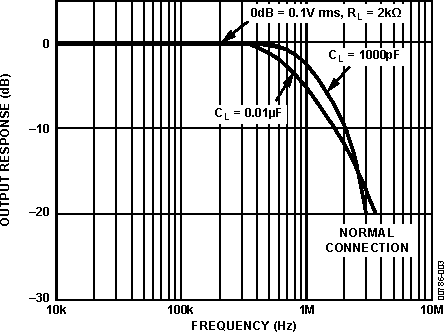
\includegraphics[scale=1]{Immagini/ad633_bp.pdf}
		\caption{Banda passante del moltiplicatore analogico AD633}
		\label{fig:sch_ad633}
	\end{figure}

	
	\noindent La \textit{Figura \ref{fig: AD633 schema a blocchi}} mostra sia il pinout che lo schema  blocchi interno dell'\textit{AD6333}.
	Il segnale in uscita dal mixer si calcola con la seguente equazione:

	\begin{equation}
		\label{eq: funzione trasferimeto AD633}
		W = \frac{(X1 - X2)(Y1 - Y2)}{10 [V]}  + Z 
	\end{equation}

	L'\textit{Equazione \ref{eq: funzione trasferimeto AD633}} ci dice che il segnale viene attenuato di un fattore 10, quindi sarà necessaria una compensazione negli stadi successivi come viene mostrato nella \textit{Sezione \ref{sec:filtro_hp1}}. 

	\noindent Analizzando il caso che gli ingressi X2, Y2 e Z collegti a massa, ovvero che diano contributo nullo. L'\textit{Equazione \ref{eq: funzione trasferimeto AD633}} diventa:


	\begin{equation}
		\label{eq: prodotto sinusoidi AD633}
		W = \frac{X1 * Y1}{10 [V]}
	\end{equation}


	Considerando che i due ingressi siano sinusoidali:

	\begin{equation}
		\label{eq: X1 sinusoidale}
		X1 = A\sin (\omega _1t + \varphi _1)
	\end{equation}
	\begin{equation}
		\label{eq: XY sinusoidale}
		Y1 = B\sin (\omega _2t + \varphi _2)
	\end{equation}
	\begin{equation}
		\label{eq:prodotto sinusoidi con fase}
		W = \frac{AB}{2}[\cos ((\omega _1 - \omega _2)t + (\varphi _1 - \varphi _2)) - \cos ((\omega _1 +\omega _2)t + (\varphi _1 + \varphi _2))]\frac{1}{10[V]}
	\end{equation}


	Aggiungendo l'ipotesi che le due sinusoidi abbiano fase nulla, l'\textit{Equazione \ref{eq:prodotto sinusoidi con fase}} diventa:


	\begin{equation}
		\label{eq:prodotto sinusoidi}
		W = \frac{AB}{2}[\cos ((\omega _1 - \omega _2)t) - \cos ((\omega _1 +\omega _2)t)]\frac{1}{10[V]} 
	\end{equation}
	

	Dunque, all'uscita del mixer si avrà un segnale dato dalla combinazione delle due sinusoidi in ingresso, le cui componenti spettrali saranno date una dalla somma delle componenti spettrali delle delle singole e l'altra dalla loro differenza.
	Quindi, inserendo un opportuno filtro passa basso, si va a selezionare solo la componente spettrale d'interesse ovvero quella compresa tra 20 $Hz$ e 20 $kHz$.

	
	\begin{figure}[H]
		\centering
		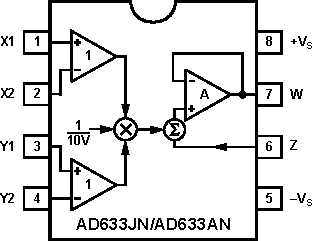
\includegraphics{Immagini/ad633_pinout.pdf}
		\caption{PinOut e schema a blocchi dell'AD633}
		\label{fig: AD633 schema a blocchi}
	\end{figure}


\chapter{Scelte progettuali}
	\label{ch:scelte}
	
	Nella realizzazione di questo progetto si deve prestare particolare attenzione allo spettro delle frequenze del segnale di uscita. Nello specifico, si deve valutare la distorsione armonica totale (\textit{THD}) del segnale di uscita osservando quanto le armoniche a frequenza diversa da quella desiderata, anche generate da disturbi intrinsechi del sistema, influiscano sovrapponendosi all'armonica a frequenza desiderata.
	Per ridurre l'effetto delle armoniche a frequenza esterna alla banda udibile si è scelto di introdurre cascate di filtri passa alto e passa basso in modo da creare un insieme di filtri passa-banda che producano un effetto accettabile per l'esperienza. Di seguito è riportato lo schema a blocchi del sistema:

	\begin{figure}[h]
		\centering
		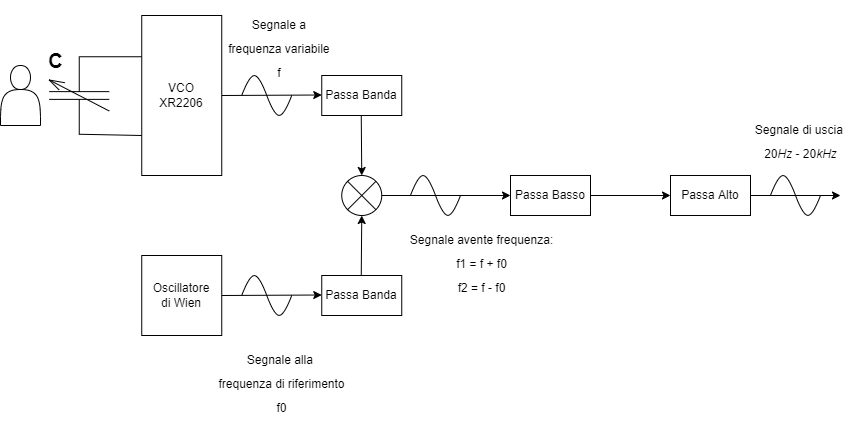
\includegraphics[scale=0.5]{Immagini/Schema a blocchicompleto giusto ita.png}
		\caption{Schema a blocchi del sistema realizzato}
		\label{fig: Schema a blocchi finale}
	\end{figure}
\space
	\noindent Nelle \textit{Sezioni \ref{sec:VCO} \ref{sec:osc_wien} \ref{sec:AD633} \ref{sec:LP4}} vengono analizzate singolarmente le scelte effettuate per ogni singolo blocco del sistema.
	 
\section{VCO}
	\label{sec:VCO}
	Il VCO, \textit{Voltage Controlled Oscillator}, è un generatore di segnali che modifica la frequenza di oscillazione del segnale generato in funzione della tensione applicata al suo ingresso.
	
	\noindent In relazione all'integrato utilizzato, il cui schema interno è riportato in figura \textit{Figura \ref{fig:sch_xr2206_}}, la frequenza di oscillazione $f_0$ viene controllata da una capacità esterna C, detta capacità di $timing$ collegata tra i \textit{pin5} e $pin6$ e dalla resistenza R posta in ingresso ai $pin7$ e $pin8$. Essa viene calcolata come:
	
	\begin{equation}
		\label{eq:freq_operation}
		f_0 = \frac{1}{RC} 
	\end{equation}

	\noindent Regolando il valore di \textit{R}, dato dalla somma di $R_1 + 1k\Omega$, e di \textit{C}, si imposta a piacere la frequenza di oscillazione.
	Nel progetto si è scelto di utilizzare una resistenza \textit{R} fissa in quanto si ha una capacità variabile per la regolazione della frequenza.

	\begin{figure}[h]
		\centering
		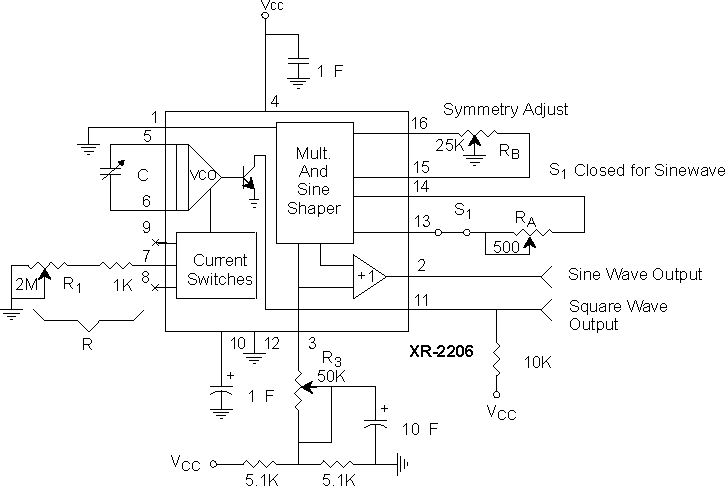
\includegraphics[scale=1]{Immagini/schema_xr2206.pdf}
		\caption{Schema a blocchi interno dell'oscillatore monolitico XR2206}
		\label{fig:sch_xr2206_}
	\end{figure}
	\newpage

	\noindent
	Come consigliato da datasheet, per garantire una buona stabilità in temperatura, si è scelto di utilizzare valori di R compresi tra $4k\Omega < R < 200k\Omega$ e valori di C compresi tra $1\mu F < C < 100\mu F$.
	
	\noindent Avendo una capacità variabile, in quanto dipendendente dalla posizione della mano dell'utente e dalla geometria dell'antenna realizzata, si è scelta una R di $100k\Omega$ per cercare di rispettare, almeno in parte, il range fornito dal datasheet per garantire una buona stabilità in temperatura. 

	
\section{Oscillatore sinusoidale di Wien}
	\label{sec:osc_wien}
	Per la realizzazione di un segnale sinusoidale a frequenza fissata si è scelto di utilizzare un oscillatore in configurazione a ponte di Wien auto-avviante, il cui schema è riportato in \textit{Figura \ref{fig:sch_osc_wien}}
	
	\begin{figure}[h]
		\centering
		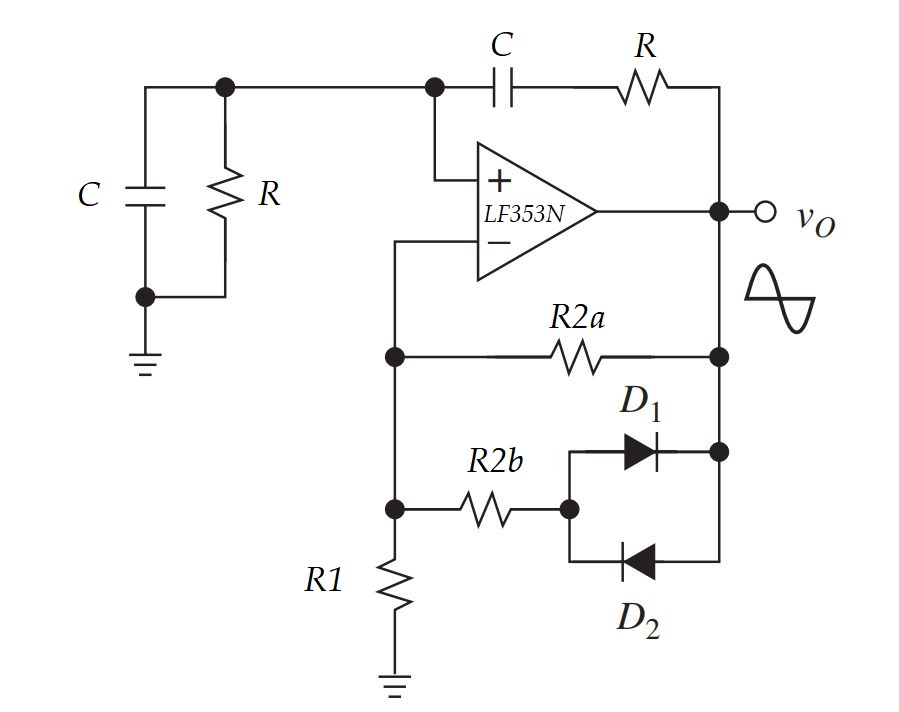
\includegraphics[scale=0.4]{Immagini/sch_osc_wien.jpg}
		\caption{Schema generale di un oscillatore a ponte di Wien auto-avviante. A sinistra lo schema utilizzato per il progetto.}
		\label{fig:sch_osc_wien}
	\end{figure}

	\noindent Analizzando la $f.d.t$ del circuito, riportata nell'equazione \ref{eq: fdt wien} si osserva che il prodotto $A\cdot B$ deve essere 1, overo che sia soddisfatta la condizione di risonanza \textit{$\omega = \omega_0$}.
 
	\begin{equation}
		\label{eq:LF356_Gain}
		T(j\omega) = \frac{1 + \frac{R_2}{R_1}}{3 + j(\frac{\omega}{\omega_0} - \frac{\omega_0}{\omega})}
		\label{eq: fdt wien}
	\end{equation}

	Il blocco di forward A è rappresentato dal guadagno del circuito ovvero:

	\begin{equation}
		\label{eq:LF356_Gain}
		A = 1 + \frac{R_2}{R_1}
	\end{equation}


	Mentre, in presenza di $R$ e $C$ di valore unico, il blocco di feedback B è rappresentato dall'equazione:
	\\
	\begin{equation}
		\label{eq:LF356_Feedback}
		B = \frac{1}{3 + j\omega RC  - j\frac{1}{\omega RC}}
	\end{equation}
	\\

	Da questo si possono avere tre casi:
	\begin{enumerate}
		\item \textit{$T(j\omega) < 1$}: si ha una situazione stabile, in cui i segnali tendono a zero. Perché si hano due poli complessi coniugati a parte reale negative, che danno origine ad una sinusoide smorzata esponenzialmente.
		\item \textit{$T(j\omega) > 1$}: si ha una situazioneinstabile, dove ogni disturbo con contributo spettrale vicino ad \textit{$\omega_0$} viene amplificato rigenerativamente. Pertanto l'amplificatore operazionale satura. Questo avviene percé si hanno due poli complessi coniugati a parte reale positiva, che danno origine ad una sinusoide con ampliezza crescente esponenzialmente.
		\item \textit{$T(j\omega) = 1$}: si ha una situazione di stabilità. Perché si hanno due poli complessi coniugati a parte reale nulla, immaginari puri, che danno origine ad una sinusoide con ampiezza costante.
	\end{enumerate}





	Per l'innesco delle oscillazioni è necessario che il guadagno ad anello aperto sia inizialmente $A\cdot B>1$ ed $A>3$ per poi assestarsi a $A\cdot B=1$ ed $A=3$. La tecnica più semplice consiste nel disporre due diodi in antiparallelo lungo l'anello di retroazione dell'amplificatore operazionale.
	
	\noindent Quando \textit{$V_{O}$} è bassa i diodi presentano un'alta resistenza differenziale mentre all'aumentare di \textit{$V_{O}$} essa diminuisce. 
	\\ Per rispettare le condizioni di lavoro imposte, il guadagno A deve essere posto, circa, all'85\% del suo valore nominale (A=2,5 — 2,55) così si fa in modo modo che $A>3$ all'avvio che poi si riduce ad A=3 a regime.

	\begin{figure}[H]
		\centering
		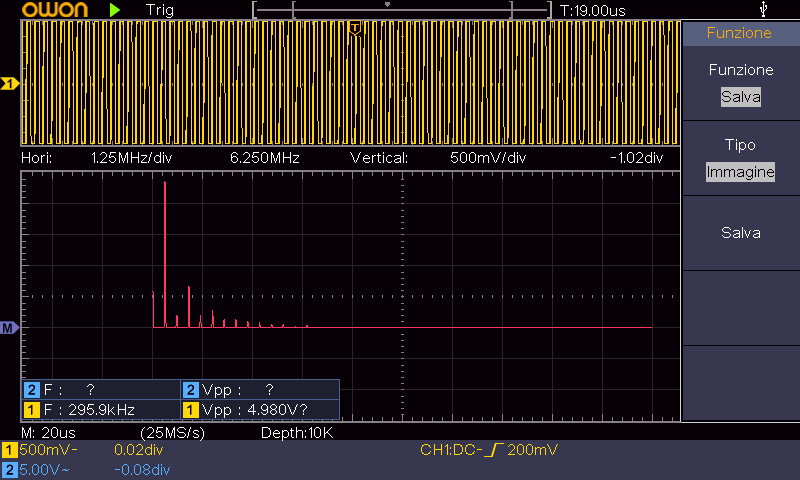
\includegraphics[scale=0.9]{Immagini/009_OscillatoreWienFFT.png}
		\caption{FFT della sinusoide a 295kHz in uscita dall'oscillatore acquisita tramite oscilloscopio}
		\label{fig:FFT295k}
	\end{figure}
	
	\noindent La frequenza di oscillazione si ottiene con l'\textit{Equazione \ref{eq:osc_wien}}:
	\begin{equation}
		\label{eq:osc_wien}
		f_0 = \frac{1}{2\pi RC}
	\end{equation}
	
	\noindent Per la valutazione della distorsione della sinusoide ottenuta si utilizza il calcolo del THD riportato nell'\textit{Equazione \ref{eq:thd}}:
	
	\begin{equation}
		\label{eq:thd}
		THD (\%) = 100 \cdot \frac{\sqrt{\sum_{2}^{\infty} V_{n}^2}}{V_1}
	\end{equation}

	\noindent Tutti i valori di tensione devono essere in RMS: 
	
	\begin{equation}
		\label{eq:Vrms}
		V_{RMS} = \frac{V}{\sqrt{2}}
	\end{equation}

	\noindent La presenza di un \textit{THD} più o meno accettabile è indice di un andamento sinusoidale in uscita più o meno ideale, ossia avente una \textit{fft} che presenta una sola riga spettrale. L'aggiunta di nuove armoniche può essere cuasata dalla sensibilità alle temperature dell'oscillatore di Wien, che porta anche ad una variazione delle ampiezze. Un'altra possibile fonte di disturbi e/o distorioni è la saturazione dell'amplificatore utilizzato per realizzare l'oscillatore, bisogna quindi essere sempre attenti a non portare l'amplificatore a saturare il segnale.


	% Se la distorsione non è armonica cosa succede? Ottendo piu righe spettrali che mi generano disturbi nel segnale
	
	% Cosa succede se la distorsione è sull'amplificatore, piuttosto che sull'oscillatore piuttosto che sull'XR? Bisogna che i componenti siano a bassa distorsione armonica.
	
	% Se il segnale in uscita all'oscillatore di wien fosse triangolare, cosa accade dopo il motiplicatore? Prossima lezione si vedrà cosa accade se il segnale è un onda quadra.
		
\newpage
\section{Moltiplicatore analogico}
	\label{sec:analog_multiplier}
	Come segue dalla teoria dei segnali, alla moltiplicazione di due segnali nei tempi corrisponde la convoluzione degli stessi in frequenza. Questo porta ad ottenere due sinusoidi centrate a frequenza $\omega_1 + \omega_2$ e $\omega_1 - \omega_2$.
	
	\noindent In \textit{Figura \ref{fig:FFTmixer}} viene mostrato il risultato ottenuto moltiplicando una sinusoide ottenuta precedentemente con l'oscillatore di Wien, illustrato nella \textit{Sezione \ref{sec:osc_wien}}, avente una $\omega_0$ di \textit{45kHz}, e una sinusoide generata dal generatore di funzione ad una frequenza di \textit{20kHz}.

	\begin{figure}[H]
		\centering
		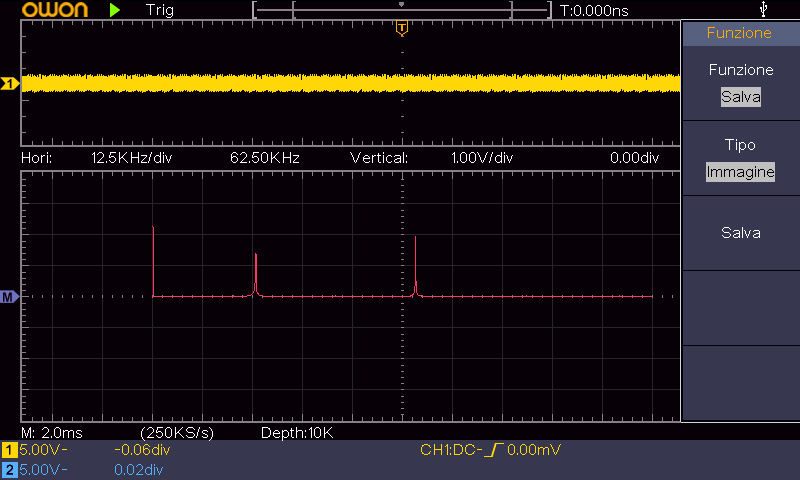
\includegraphics[scale=0.9]{Immagini/uscita_ad633_con_fcngen_20k_e_osc_45k.png}
		\caption{FFT del segnale in uscita dall'AD633, con test tra Oscillatore di Wien avente $\omega_0$ = 45kHz 12V picco e generatore di funzione con segnale 20 Khz e 2.5V picco.}
		\label{fig:FFTmixer}
	\end{figure}
	
	 \noindent Essendo i due segnali di 20kHz e 45kHz rispettivamente, dalla \textit{Figura \ref{fig:FFTmixer}} si può notare come vengano generate due sinusoidi aventi armoniche fondamentali a $(45-20)kHz$ e $(45+20)kHz$. 
	 \\
	 Inoltre, le ampiezze misurate risultano comparabili con i risultati teorici in quanto l'ampiezza di picco dei due segnali è di \textit{12V} e \textit{2.5V} rispettivamente, che vengono moltiplicati tra loro e scalati di un fattore $10$, come specificato nel datasheet del componente. Sempre in riferimento alla \textit{Figura \ref{fig:FFTmixer}} si può notare anche come le due ampiezze non siano uguali: questo è un errore dovuto alla non-linearità del componente. Tuttavia, per la nostra applicazione questo errore è irrilevante in quanto interessa maggiormente la componente frequenziale del segnale.
	

\section{Filtro LP del quarto ordine}
	\label{sec:LP4}
	Il prodotto di due sinusoidi del mixer porterà in uscita due sinusoidi a frequenze diverse ovvero una sarà $\omega_{wien} + \omega_{VCO}$ e l'altra a $\omega_{wien} - \omega_{VCO}$. Per rientrare nelle specifiche di progetto, è stato necessario introdurre un filtro passa-basso che permetta di ottenere in uscita al sistema solo la componente armonica $\omega_{wien} - \omega_{VCO}$.
	\\ 
	Volendo realizzare un filtro molto selettivo e, avendo il componente \textit{LF353P} al suo interno due amplificatori, si è scelto di utilizzare un filtro attivo di ordine 4, realizzandolo tramite un filtro di Chebychev con due celle Sallen-Key in casacata. 
	
	\begin{figure}[H]
		\centering
		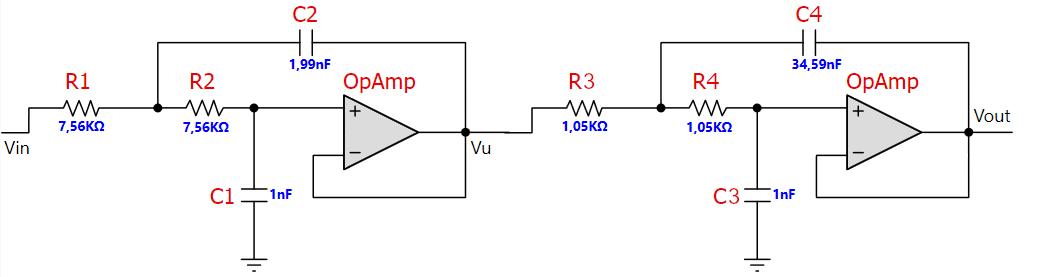
\includegraphics[scale=0.9]{Immagini/sch_lp4.png}
		\caption{Filtro attivo di ordine 4.}
		\label{fig:LP4}
	\end{figure}	
	
	\noindent La risposta in frequenza teorica del filtro risulta essere in modulo quella riportata nel diagramma di Bode mostrato in \textit{Figura \ref{fig:BodeLp4}}.
	
	\begin{figure}[H]
		\centering
		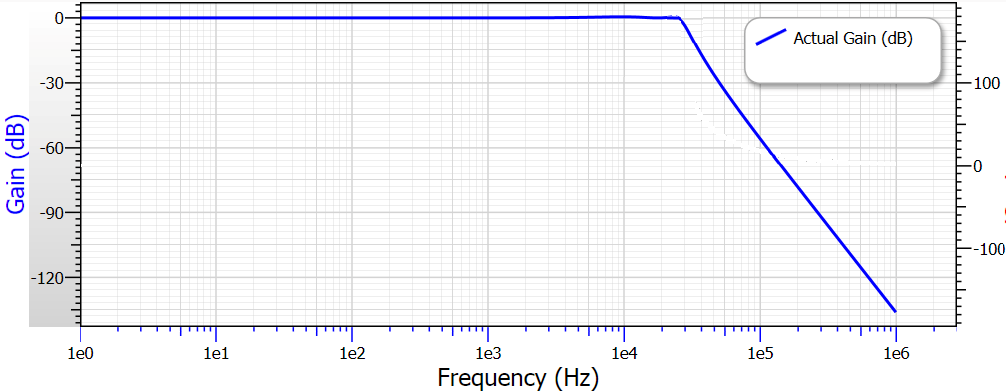
\includegraphics[scale=0.9]{Immagini/bode_teorico_lp4.png}
		\caption{Diagramma di Bode del modulo del filtro.}
		\label{fig:BodeLp4}
	\end{figure}

	La funzione di trasferimento del filtro del quarto ordine può essere vista come il prodotto in cascata delle funzioni di trasferimeto delle due celle Sellen-Key del secondo ordine.

	La funzione della prima cella risulta:

	\begin{equation}
		\label{eq:sallen-key-1}
		H_1(s) = \frac{V_{in}}{V_u}  =  \frac{1}{1 + sC_1(R_1 + R_2)+ s^2C_1C_2R_1R_2 } 
	\end{equation}

	Mentre la funzione di trasferimento della seconda cella risulta essere:

	\begin{equation}
		\label{eq:sallen-key-2}
		H_2(s) = \frac{V_u}{V_{out}}  = \frac{1}{1 + sC_3(R_3 + R_4)+ s^2C_3C_4R_3R_4 } 
	\end{equation}

	La funzione di trasferimento totale del filtro sarà quindi data dal prodotto delle due \textit{Equazioni \ref{eq:sallen-key-1}e \ref{eq:sallen-key-2}}:

	\begin{equation}
		H(s) = H_1(s)H_2(s) =  \frac{V_{in}}{V_u}\frac{V_u}{V_{out}} = \frac{V_{in}}{V_{out}}
	\end{equation}

	\section{Filtro passa alto del primo orine con amplificazione}
	\label{sc: pasas alto teoria}
	Come mostrato nello schema riportato in figura \ref{fig: Schema a blocchi finale}, il sistema presenta come ultimo blocco un filtro passa alto, per tagliare tutte le frequenze inferiori ai 20 \textit{Hz}, come da specifica. Inoltre, oltre a filtrare le basse frequenze si effettua anche un'amplificazione per compensare il fattore di attenuazione introdotto dal mixer.
	\begin{figure}[H]
		\centering
		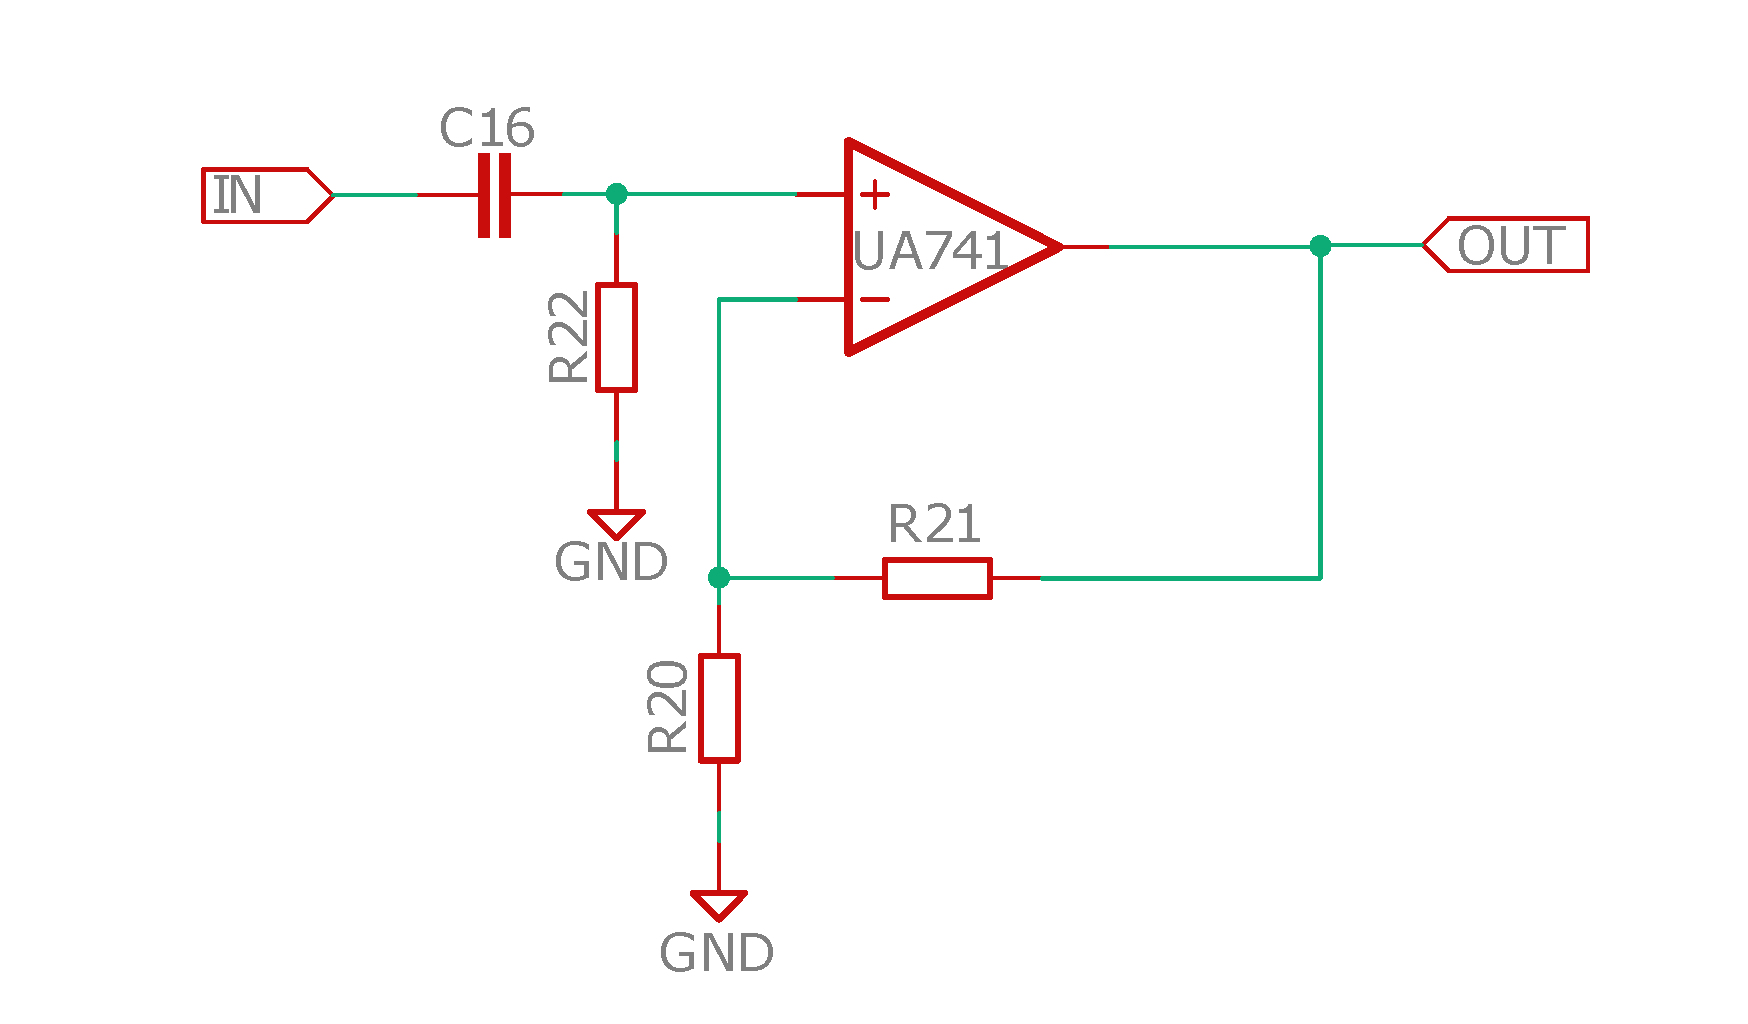
\includegraphics[scale=0.4]{Immagini/sch_hp1_no_valori.pdf}
		\caption{Schematico del filtro passa alto attio del primo ordine, con guadagno per compensare l'attenuazioen itordotta dal mixer. Posto in uscita dal filtro passa basso del quarto ordine.}
		\label{fig:FiltroH1Pnoval}
	\end{figure}

La funzione di trasferimetno del filtro può essere vista come il prodotto di due dieversi blocchi. Il blocco di guadagno non invertente riportato nell'equazione \ref{eq:gain passa alto}, ovveor il blocco di retroazione. Che per compensare il fattore di attenuazione introdotto dal mixer il guadagno dovrà essere pari a 10. 

\begin{equation}
	\label{eq:gain passa alto}
	A = 1 + \frac{R_2}{R_1}
\end{equation}

Il secondo blocco invece conprende la parte di filtraggio e la sua funzione di trasferimento è quella riportata nell'eqauzione \ref{eq:fdt passa alto}.

\begin{equation}
	\label{eq:fdt passa alto}
	H(j\omega) = \frac{j\omega RC}{1 + j\omega RC}
\end{equation}

Moltiplicando l'equazione \ref{eq:gain passa alto} con l'equazione \ref{eq:fdt passa alto} e passando nel dominio di Laplace, ovvero ponendo \textit{$j\omega = s$}, si ottine la finzione di trasferimento complessiava del filtro attivo riportata nell'equazione \ref{eq:fdt passa alto + gain}.

\begin{equation}
	\label{eq:fdt passa alto + gain}
	H(s) = \frac{sRC}{1 + sRC}(1 + \frac{R_2}{R_1})
\end{equation}

La frequenza di taglio si ottine con la formula riportata nell'equazione \ref{eq:taglio passa alto}

\begin{equation}
	\label{eq:taglio passa alto}
	f_t = \frac{1}{2\pi RC}
\end{equation}

Imponendo una \textit{C} pari a \textit{$47nF$}, per ottenere una $f_t$ pari a \textit{20 Hz}, si deve avere una \textit{R} pari a \textit{$169.3k\Omega$}.

\section{Filtro passa banda passivo}
\label{sc: passa banda teoria}
Anche se nello schema riportato in figura \ref{fig: Schema a blocchi finale} i filtri passa banda vengono posti all'inizio, sono stati messi come ultimo sezione in quanto la loro necessità si è presentata solo dopo una prima anlisi dei segnali in uscita dall'XR2206 edall'oscillatore riportato nella sezione \ref{subsc: wien sbagliato}. 
\noindent Visto che i due segnali impiegati nella misurazioni presentavano delle componenti in continua, sopratutto il segnale in uscita dall'XR2206 che introduce un offset per garantire l'oscillazione con un'alimetazione singola, come spiegato nella sezione \ref{sec:XR2206}; mentre l'oscillatore nella sezione \ref{subsc: wien sbagliato} si presentava con un pessimo \textit{THD} dovuto alla presenza di diverse aroniche indesiderate. Quindi, al fine di evitare la comparsa di più armoniche indesiderate in uscita dal mixer si è deciso di introdurre il filtro passa banda passivo riportato in figura \ref{fig:FiltroBP}.


\begin{figure}[H]
	\centering
	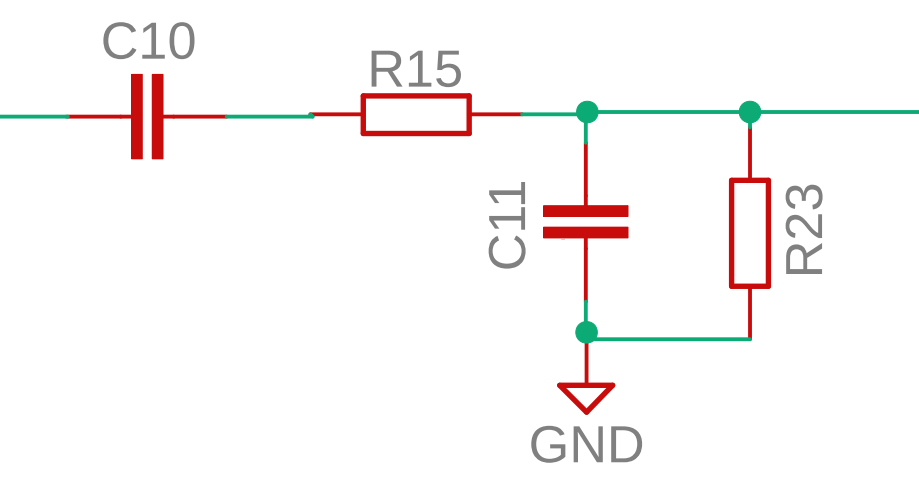
\includegraphics[scale=0.25]{Immagini/sch_crc_no_valori.png}
	\caption{Schematico del filtro passa banda passivo meso in uscita dal XR2206 e in uscita all'oscillatore riportato nel paragrafo \ref{subsc: wien sbagliato}}
	\label{fig:FiltroBP}
\end{figure}

La funzione di trasferimento del filtro è riportata nell'equazione \ref{eq:fdt passa banda teo}.

\begin{equation}
	\label{eq:fdt passa banda teo}
	H(s) = \frac{\frac{s}{C_2R_1}}{s^2 + s(\frac{1}{C_2R_2} + \frac{1}{C_1R_1} + \frac{1}{C_2R_1}) + \frac{1}{C_2R_2C_1R_1}}
\end{equation}

Si possono notare due poli il primo in \textit{$kHz$} e il secondo in \textit{$kHz$} e di uno zero nell'origine. Questi garantiscono il filtraggio della continua come desiderato ed una prima attenuazione delle frequenze oltre il valore massimo che consente di demodulare in uscita la sinusoide con la frequenza compresa nell'intervallo imposto dalle specifiche.

Si può notare la presenza di un patitore di tensione. Per evitare un attenuazione del segnale si è deciso di iporre $R_2$ molto maggiore di $R_1$ in modo che l'equazione del partitore di tensione, riportato nell'equazione \ref{eq: partitore di tensione}, diventi l'equazione \ref{eq: partitore di tensione circa 1}.

\begin{equation}
	V_{out} = V_{in} \frac{R_1}{R_1 + R_2}
	\label{eq: partitore di tensione}
\end{equation}

\begin{equation}
	V_{out} \sim  V_{in}   se   R_1 >> R_2
	\label{eq: partitore di tensione circa 1}
\end{equation}

In figura \ref{fig:BodeBP} riporta il diagrama di Bode del modulo relativo al filtro passa banda progettato.

\begin{figure}[H]
	\centering
	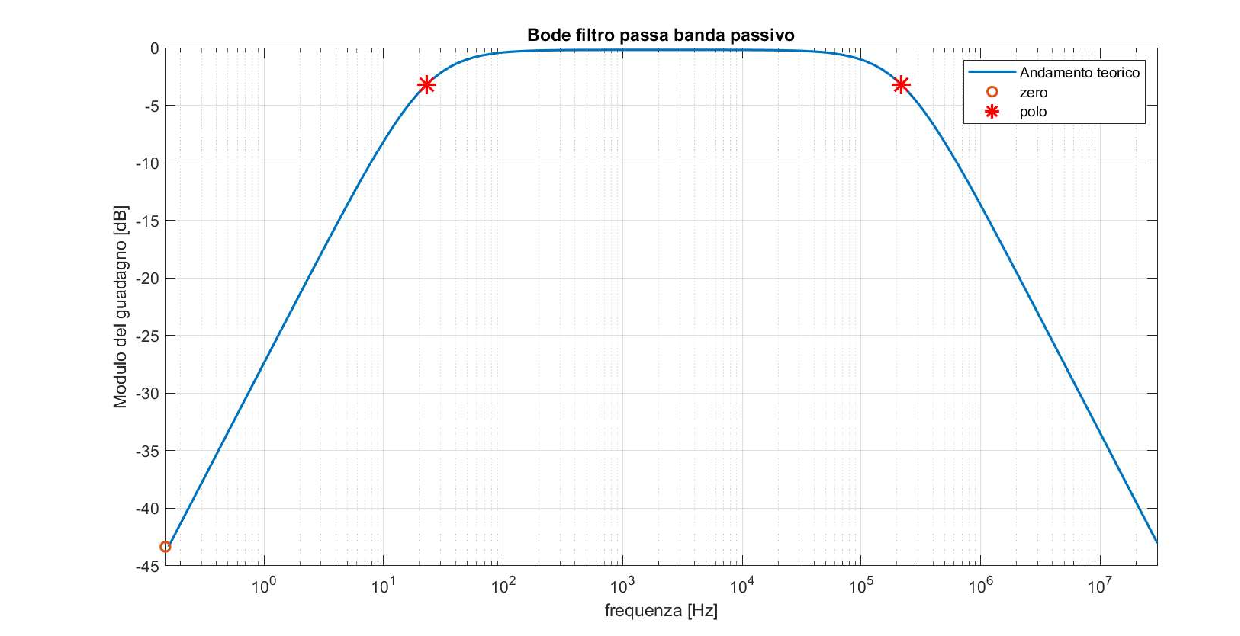
\includegraphics[scale=0.8]{Immagini/bode_filtro_passa_banda_matlab.pdf}
	\caption{Diagramma di Bode del filtro passa banda passivo con evidenziati il polo e gli zeri.}
	\label{fig:BodeBP}
\end{figure}
	
\chapter{Risultati sperimentali}
\label{ch:Risultati_sperimentali}
\section{XR2206}
	Per la realizzazione della sinusoide a frequenza variabile si è fatto riferimento al datasheet del componente scegliendo come valori di partenza quelli mostrati in esempio. 
	La capacità variabile è stata realizzata con un supporto rigido e della carta di alluminio creando una struttura simile ad una bandiera. Il tutto è stato collegato come mostrato in \textit{Figura \ref{fig:antenna}}.

	\begin{figure}[H]
		\centering
		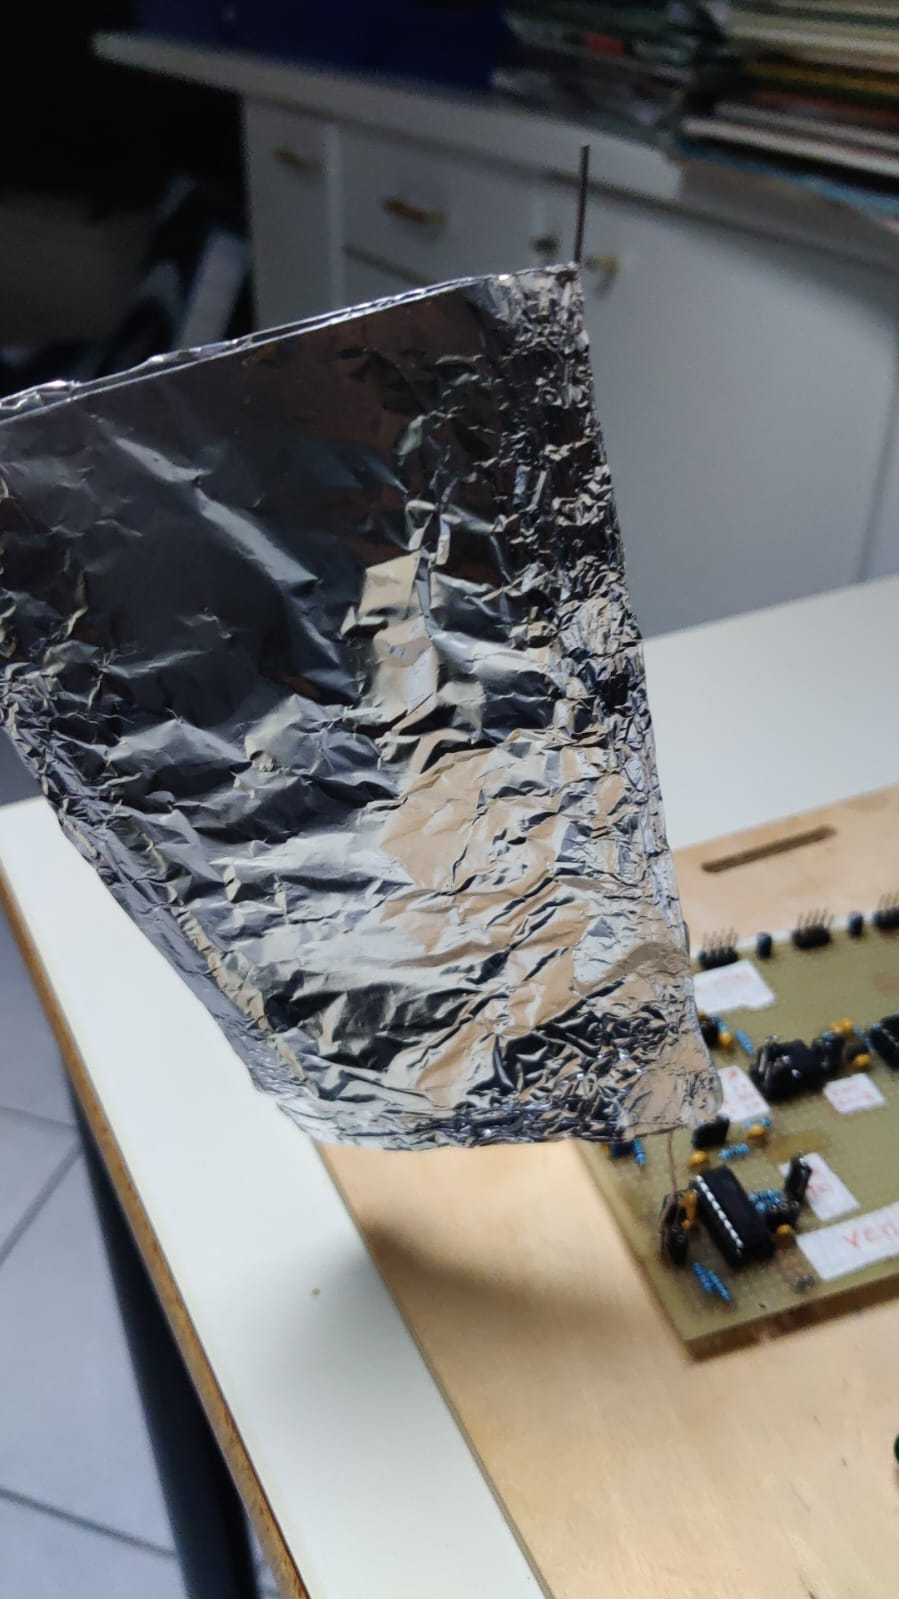
\includegraphics[scale=0.25]{Immagini/Antenna.jpg}
		\caption{Foto dell'antenna utilizzata come capacità variabile}
		\label{fig:antenna}
	\end{figure}
	
	Le prestazioni ottenute con questo tipo di antenna sono mostrate in \textit{Figura \ref{fig:SINxr+LP}} e in \textit{Figura \ref{fig:SINx}}. Dalle figure si può osservare le sinusoidi in uscita dall'XR2206 in presenza dell'antenna a bandiera e in assenza della mano dell'utente, ovvero l'oscillazione a \textit{"riposo"} dell'oscillatore. È importante notare come dalla \textit{Figura \ref{fig:SINx}} venga evidenziata l'attenuazione e lo sfasamento del segnale dovuti all'effetto del filtro passa banda. Tuttavia, il filtro migliora le prestazioni di uscita dell'oscillatore. Infatti, già dalla \textit{Figura \ref{fig:SINxr+LP}} si può apprezzare la buona riuscita del sistema in termini di segnale sinusoidale generato. Prestazioni che possono essere quantificate con un'analisi di tipo spettrale.

	\begin{figure}[H]
		\centering
		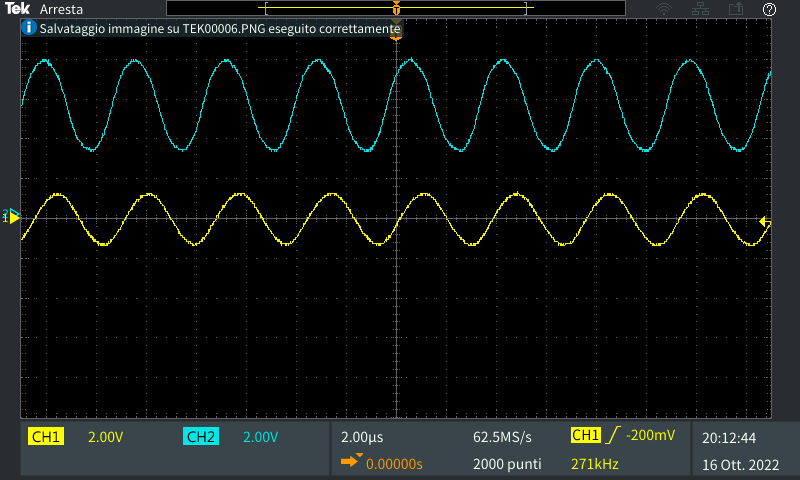
\includegraphics[scale=0.5]{Immagini/sin_xr+lp.PNG}
		\caption{Confronto tra i segnali in uscita dall'oscillatore monolitico XR2206 prima (in bianco) e dopo (in giallo) il fitro LP in cascata.}
		\label{fig:SINxr+LP}
	\end{figure}


	\begin{figure}[H]
		\centering
		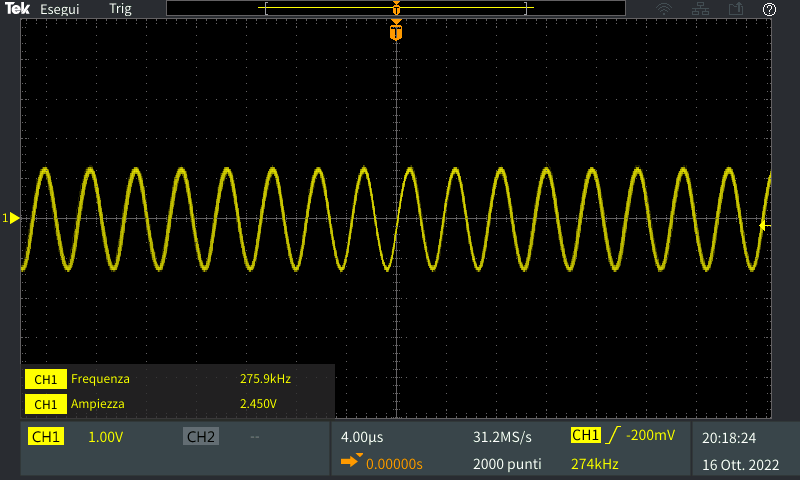
\includegraphics[scale=0.5]{Immagini/sin_xr.PNG}
		\caption{Segnale in uscita dal blocco XR2206 + LP.}
		\label{fig:SINx}
	\end{figure}

	La figura \ref{fig:FFTxr+LP} mostra la \textit{FFT} in uscita dall'\textit{XR2206} prima del filtro (segnale in bianco) e dopo il filtro (segnale in giallo). I due segnali oscillano alla stessa frequenza fondamentale e sono stati visualizzati con scala differente per poterne apprezzare l'intera riga spettrale. Si nota che l'armonica dopo il filtro (in giallo) presenta un miglioramento del THD rispetto a quella non filtrata (in bianco) in quanto le armoniche a frequenza diversa dalla fondamentale vengono attenuate, anche se la riduzione in ampiezza interessa anche la fondamentale. La tabella \ref{tab:THD_XR2206+BP} mostra i valori numerici ottenuti dal calcolo del \textit{THD} sostituendo i valori numerici delle ampiezze del segnale risultante nell'\textit{Equazione \ref{eq:thd}}.

	\begin{figure}[H]
		\centering
		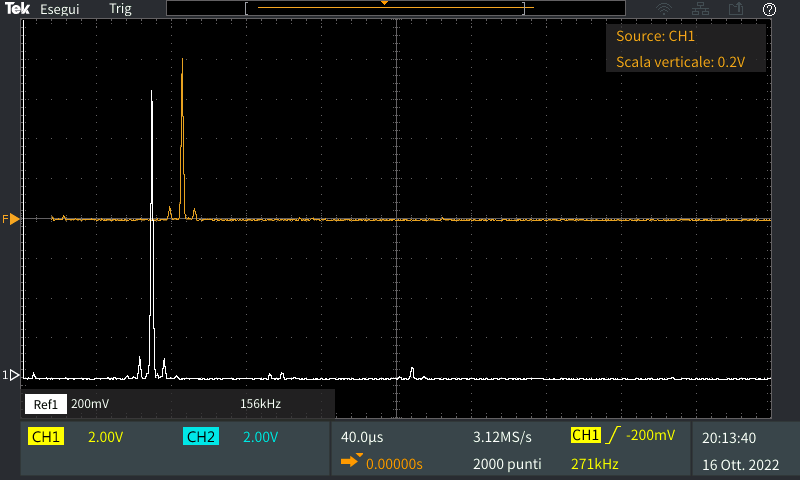
\includegraphics[scale=0.5]{Immagini/fft_xr+lp.PNG}
		\caption{Confronto tra le FFT del segnale in uscita dall'oscillatore monolitico XR2206 prima e dopo il filtro LP in cascata.}
		\label{fig:FFTxr+LP}
	\end{figure}


	\begin{table}[h!]
		\centering
		\begin{tabular}{||c|c|c||}
			\hline
			\cellcolor{gray!10}Armonica & \cellcolor{gray!10}Ampiezza [mV] & \cellcolor{gray!10}THD (\%) \\
			\hline
			Fondamentale & 800 &\\
			\cline{1-2}
			$2^a$ armonica & 40 & 7.071 \\
			\cline{1-2} 
			$3^a$ armonica & 40 & \\
			\hline	
		\end{tabular}
		\caption{Misure in ampiezza delle componenti armoniche e calcolo del THD della sinusoide in scita dall'XR2206 filtrata dal filtro passa-banda}
		\label{tab:THD_XR2206+BP}
	\end{table}

\newpage
\section{Oscillatore di Wien}
\label{sc: oscillatore wien sperimentale}


	In figura \ref{sch:osc_wien} è riportato il circuito finale utilizzato per la realizzazione dell'oscillatore di Wien.
	In figura \ref{fig:sch_osc_wien} è riportato lo schematico dell'oscillatore di Wien utilizzato per generare la sinusoide di riferimento alla frequenza di 245 \textit{kHz}. La frequenza è stata ottenuta sostituendo nell'equazione \ref{eq:osc_wien} il valore di \textit{C} pari a \textit{330pF} e una \textit{R} pari a \textit{$2 k\Omega$}. Inoltre si è scelto di usare una \textit{R2a} di \textit{2M\Omega} per garantire un passaggio di corrente tra uscita e ingresso.

	\begin{figure}[H]
		\centering
		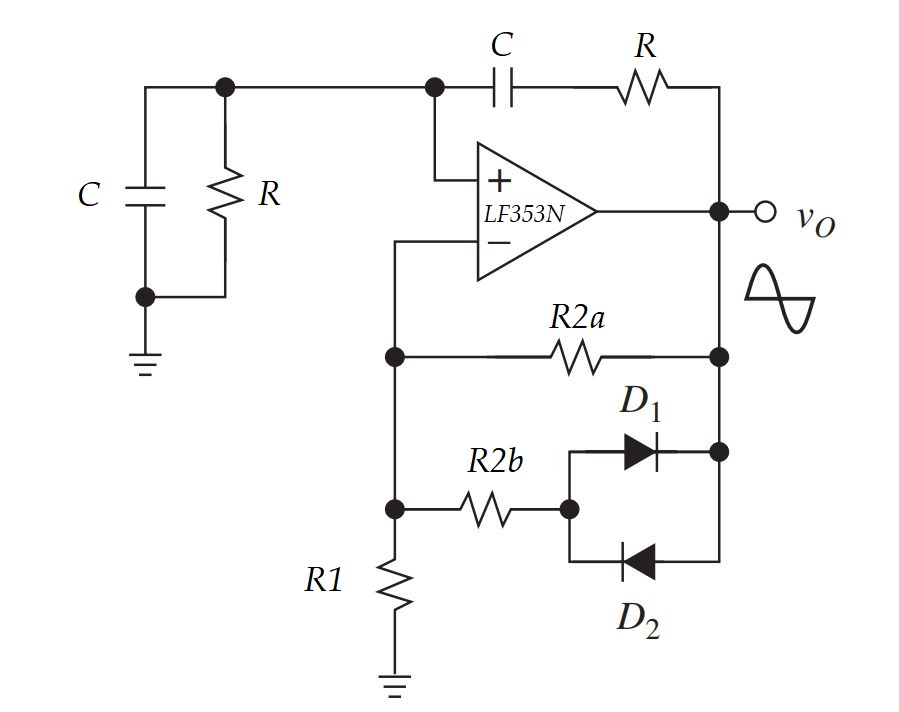
\includegraphics[scale=0.5]{Immagini/sch_osc_wien.jpg}
		\caption{Schematico dell'oscillatore di Wien utilizzato}
		\label{fig:sch_osc_wien}
	\end{figure}

	La figura \ref{fig:SINwien+BP} mostra l'uscita dell'oscillatore di Wien. In azzurro si può notare che la sinusoide satura sulla semionda negativa e le pendenze di salita a discesa sono differenti. Questo accade quando il valore di resistenza utilizzato dei potenziometri è comparabile. La saturazione del segnale di uscita dell'integrato porta all'introduzione di altre armoniche oltre alla fondamentale, come mostrato dal segnale in bianco mostrato in \textit{Figura \ref{fig:FFTwien+BP}}.

	\begin{figure}[H]
		\centering
		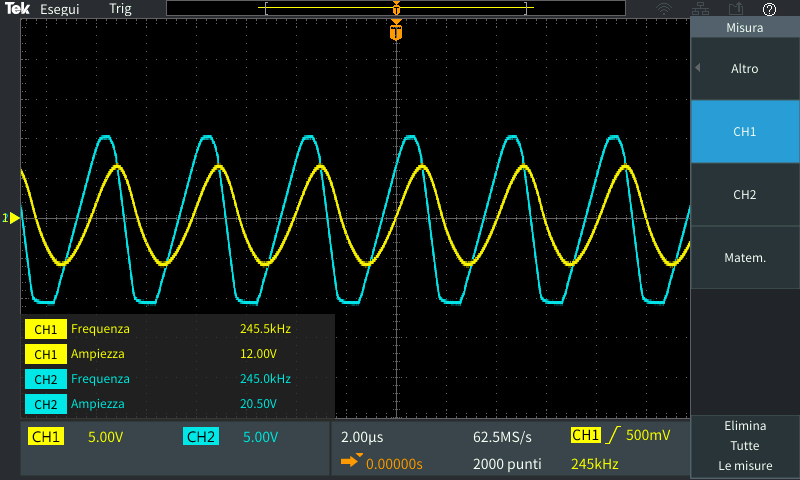
\includegraphics[scale=0.5]{Immagini/osc_wien+bp210k.PNG}
		\caption{Confronto tra i segnali in uscita dall'oscillatore di Wien prima e dopo il fitro BP in cascata.}
		\label{fig:SINwien+BP}
	\end{figure}

	Per risolvere questo problema è stato aggiunto un filtro passivo all'uscita dell'oscillatore. Il filtro è di tipo passa banda formato da un condensatore per tagliare la continua, seguito da un passa basso RC ($R = 7.5k\Omega$; $C = 100pF; f_c = 212kHz$).
	L'aggiunta di questo filtro porta un notevole miglioramento del segnale di uscita. Tale miglioramento è osservabile sia in \textit{Figura \ref{fig:SINwien+BP}} (sinusoide in giallo), dove si può notare l'assenza di saturazione delle semionde e fronti di salita e discesa pressoché identici, che in figura \ref{fig:FFTwien+BP} dove di può notare la notevole riduzione delle armoniche nello spettro del segnale.

	Tuttavia, l'aggiunta di un filtro di questo tipo porta ad un'attenuazione anche dell'armonica fondamentale e ad uno sfasamento di 90° in ritardo rispetto alla sinusoide originale. L'attenuazione è dovuta alla scelta della frequenza di taglio del filtro ($212kHz$), che quindi inizierà a tagliare circa $20/30kHz$ prima della fondamentale dell'oscillatore di Wien che è generata a $245kHz$. Lo sfasamento invece è dovuto al filtro del primo ordine passivo.

	\begin{figure}[H]
		\centering
		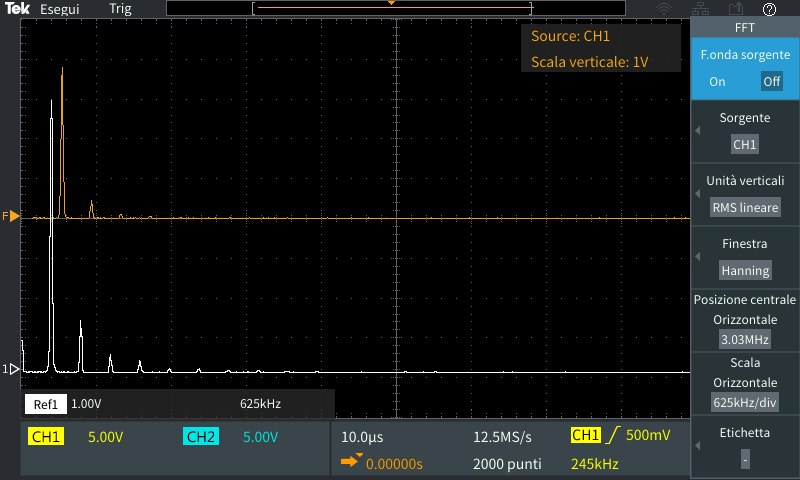
\includegraphics[scale=0.5]{Immagini/fft_osc+bp210k.PNG}
		\caption{Confronto tra le FFT del segnale in uscita dall'oscillatore di Wien prima e dopo il filtro BP in cascata.}
		\label{fig:FFTwien+BP}
	\end{figure}

	Un altro riscontro lo si ha con il calcolo del \textit{THD} del segnale in uscita dall'oscillatore il cui risultato ottenuto l'\textit{Equazione \ref{eq:thd}} è mostrato nella \textit{Tabella \ref{tab:THD_WIEN}}. Invece, nella tabella \ref{tab:THD_WIEN+LP} è riportato il valore del \textit{THD} ottenuto sempre dall'\textit{Equazione \ref{eq:thd}} riferito al segnale risultante in uscita al filtro passa banda passivo. 
	Confrontando i due risultati ottenuti, si può osservare un effettivo miglioramento del \textit{THD} della sinusoide di riferimento.

	\begin{table}[h!]
		\centering
		\begin{tabular}{||c|c|c||}
			\hline
			\cellcolor{gray!10}Armonica & \cellcolor{gray!10}Ampiezza [mV] & \cellcolor{gray!10}THD (\%) \\
			\hline
			Fondamentale & 6800 &\\
			\cline{1-2}
			$2^a$ armonica & 1200 & \\
			\cline{1-2} 
			$3^a$ armonica & 600 & 19.96 \\
			\cline{1-2} 
			$4^a$ armonica & 200 & \\
			\cline{1-2} 
			$5^a$ armonica & 50 & \\
			\hline	
		\end{tabular}
		\caption{Ampiezza delle armoniche del segnale in uscita dall'oscillatore di Wien.}
		\label{tab:THD_WIEN}
	\end{table}

	\begin{table}[h!]
		\centering
		\begin{tabular}{||c|c|c||}
			\hline
			\cellcolor{gray!10}Armonica & \cellcolor{gray!10}Ampiezza [mV] & \cellcolor{gray!10}THD (\%) \\
			\hline
			Fondamentale & 3800 &\\
			\cline{1-2}
			$2^a$ armonica & 400 & 10.61 \\
			\cline{1-2} 
			$3^a$ armonica & 50 & \\
			\hline	
		\end{tabular}
		\caption{Ampiezze delle armoniche del segnale filtrato con il filtro passa basso in cascata all'oscillatore di Wien.}
		\label{tab:THD_WIEN+LP}
	\end{table}


\section{Mixer}
\label{sec:Mixer}

	L'\textit{AD633} rappresenta il blocco del mixer nel nostro sistema. Il suo compito è moltiplicare tra loro le due sinusoidi in ingresso. Le sinusoidi interessate sono quella di riferimento dell'oscillatore di Wien e quella in uscita dal VCO. Quest'ultima sarà variabile e dipenderà dalla distanza della mano rispetto all'altro estremo della capacità variabile (bandiera in alluminio).


	Una delle problematiche riscontrate durante l'utilizzo del mixer è stata la manifestazione di un offset del segnale dovuto all'impossibilità degli ingressi di scaricare le correnti di bias verso massa. Questo ha portato alla comparsa di offset negativo e alla cancellazione delle altre armoniche in uscita.

	La soluzione si è trovata inserendo una resistenza di valore \textit{680k$\Omega$} agli ingressi del mixer, creando un percorso verso massa per le correnti di bias. La scelta di tale valore è dovuta al compromesso tra l'ingresso ad alta impedenza dell'AD633 e il partitore formato con la resistenza del filtro. La scelta di un valore errato produrrebbe un'attenuazione indesiderata del segnale di ingresso al mixer. Il resistore scelto evita l'attenuazione del segnale e salvaguarda l'alta impedenza del componente. Ciò che si è ottenuto è mostrato in \textit{Figura \ref{fig:FFTAD633}}, dove è possibile osservare il risultato della moltiplicazione di due segnali sinusoidali nel dominio delle frequenze.
	\begin{figure}[H]
		\centering
		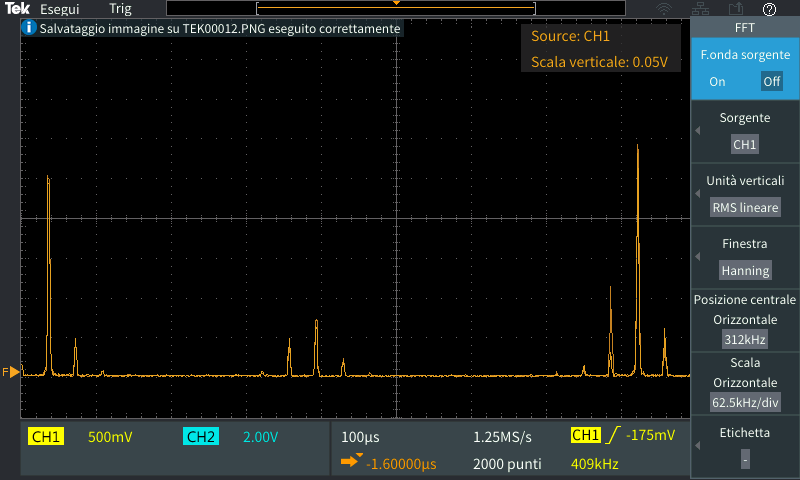
\includegraphics[scale = 0.5]{Immagini/ad633_fft_mixed.PNG}
		\caption{FFT in uscita dal mixer AD633 senza filtraggio}
		\label{fig:FFTAD633}
	\end{figure}

	Quello che si evince osservando la figura \ref{fig:FFTAD633} è che le armoniche presenti alle frequenze superiori a quelle di interesse nei due segnali e in ingresso all'integrato, visibili nelle figure \ref{fig:FFT SINwien breadboard} e \ref{fig:FFTwien+BP}, comportano la presenza delle armoniche fondamentali conseguenti al prodotto tra le due sinusoidi. Inoltre, l'ampiezza maggiore delle armoniche di alta frequenza rispetto a quelle in bassa frequenza, è dovuto alla sovrapposizione dei prodotti misti tra armoniche indesiderate e fondamentali dei segnali. In particolar modo, i prodotti in cui le frequenze si sommano, si sovrappongono a quelli in cui le frequenze si sottraggono. La figura \ref{fig:FFTAD633mark} evidenzia le armoniche citate.

	\begin{figure}
		\centering
		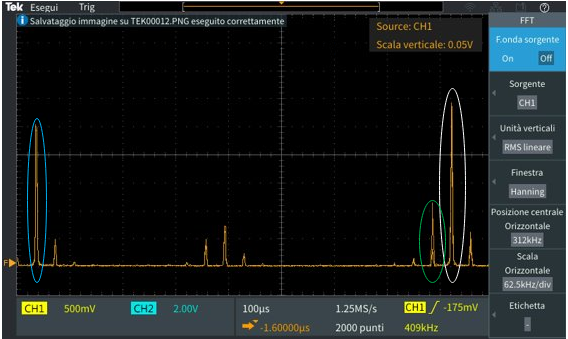
\includegraphics[scale=0.75]{Immagini/ad633_edited.png}
		\caption{Armoniche coinvolte nella sovrapposizione messe in evidenza}
		\label{fig:FFTAD633mark}
	\end{figure}

	\label{ch:Risultati}
	
\newpage
\section{Filtro passa basso di ordine 4}
	In uscita dal mixer è stato necessario inserire un filtro passa basso per eliminare le frequenze superiori ai \textit{20kHz}, come richiesto da specifica di progetto. Esso è necessario per eliminare le componenti date dalla somma delle frequenze in uscita al mixer risultanti dell'\textit{Equazione \ref{eq: prodotto sinusoidi AD633}}. Infatti, dati due segnali del tipo $ V_1 = A_1 \cdot sin(\omega_1t) $
	e $ V_2 = A_2 \cdot sin(\omega_2t) $, il segnale risultante dalla moltiplicazione analogica tra i due sarà dato dall'equazione \ref{eq:analog_multiply}:
	\begin{equation}
		V_m = V_1 \cdot V_2 = \frac{A_1A_2}{2}[sin((\omega_1 + \omega_2)t) + sin((\omega_1 - \omega_2)t)]
		\label{eq:analog_multiply}
	\end{equation}
	La figura \ref{fig:bode_LF353P} mostra il comportamento in frequenza dell'\textit{LF353P}, ovvero il componente utilizzato per la realizzazione del filtro passa basso di ordine quattro.

	\begin{figure}[h]
		\centering
		\subfloat[][\emph{Relazione picco massimo di tensione e frequenza}]
		{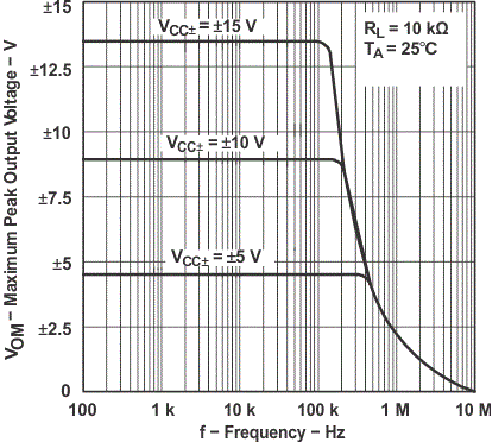
\includegraphics[width=.45\textwidth]{Immagini/lf353p_performance.pdf}} \qquad
		\subfloat[][\emph{Amplificazione della differenza di tensione degli ingressi in relazione alla frequenza}]	     	{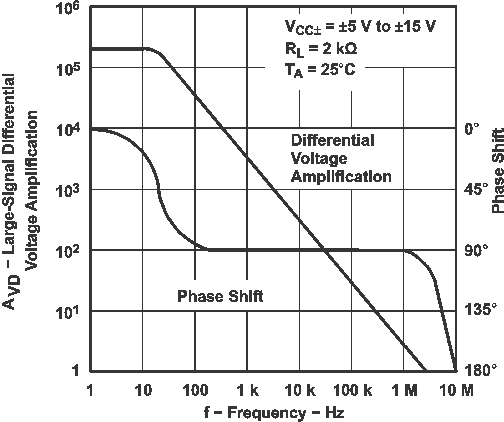
\includegraphics[width=.49\textwidth]{Immagini/bode_lf353p.pdf}} \\
		\caption{Diagrammi di bode del componente LF353P in anello aperto}
		\label{fig:bode_LF353P}
	\end{figure}

	La scelta di un filtro del quarto ordine è stata fatta sia per garantire un'atteuazione sufficiente delle armoniche successive ai \textit{20KHz} sia perché l'\textit{LF356P} contiene al suo interno due operazionali. Quindi per evitare di lasciare flottanti dei pin che sarebbero potuti diventare una fonte aggiuntiva di rumore, si è deciso di utilizzare il componente al meglio delle possibilità.
	L'andamento del filtro ottenuto è mostrato in \textit{Figura \ref{fig:BODELp4Real}}, la quale mostra che le scelte progettuali sono state corette, in quanto i dati sperimentali rispecchiano l'andamento teorico del filtro.
	Come si può osservare in \textit{Figura \ref{fig:BODELp4Real}} i due andamenti sono molto simili.
	
	\begin{figure}[H]
		\centering
		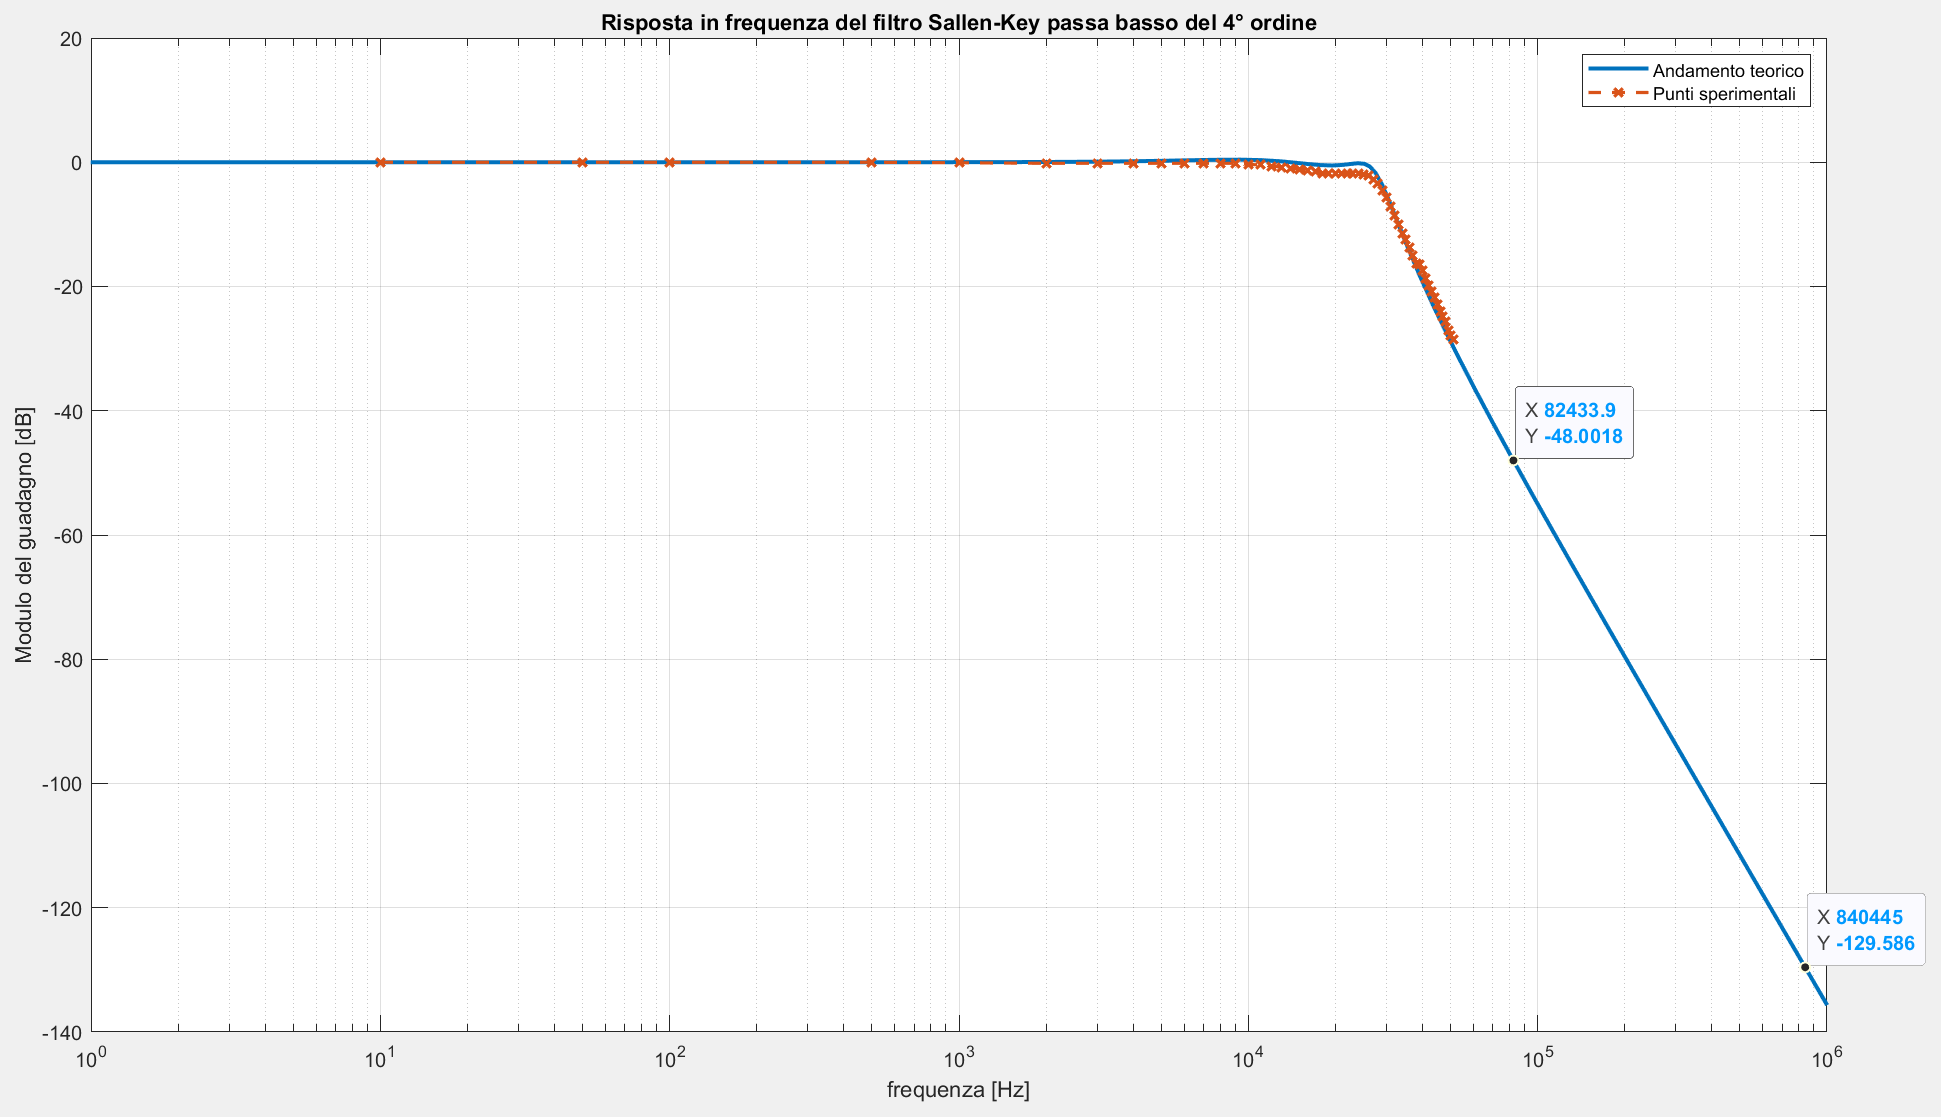
\includegraphics[scale=0.48]{Immagini/bode_lp4.png}
		\caption{Diagramma di Bode del filtro Sallen-Key del $4^o$ ordine}
		\label{fig:BODELp4Real}
	\end{figure}

	\begin{figure}[H]
		\centering
		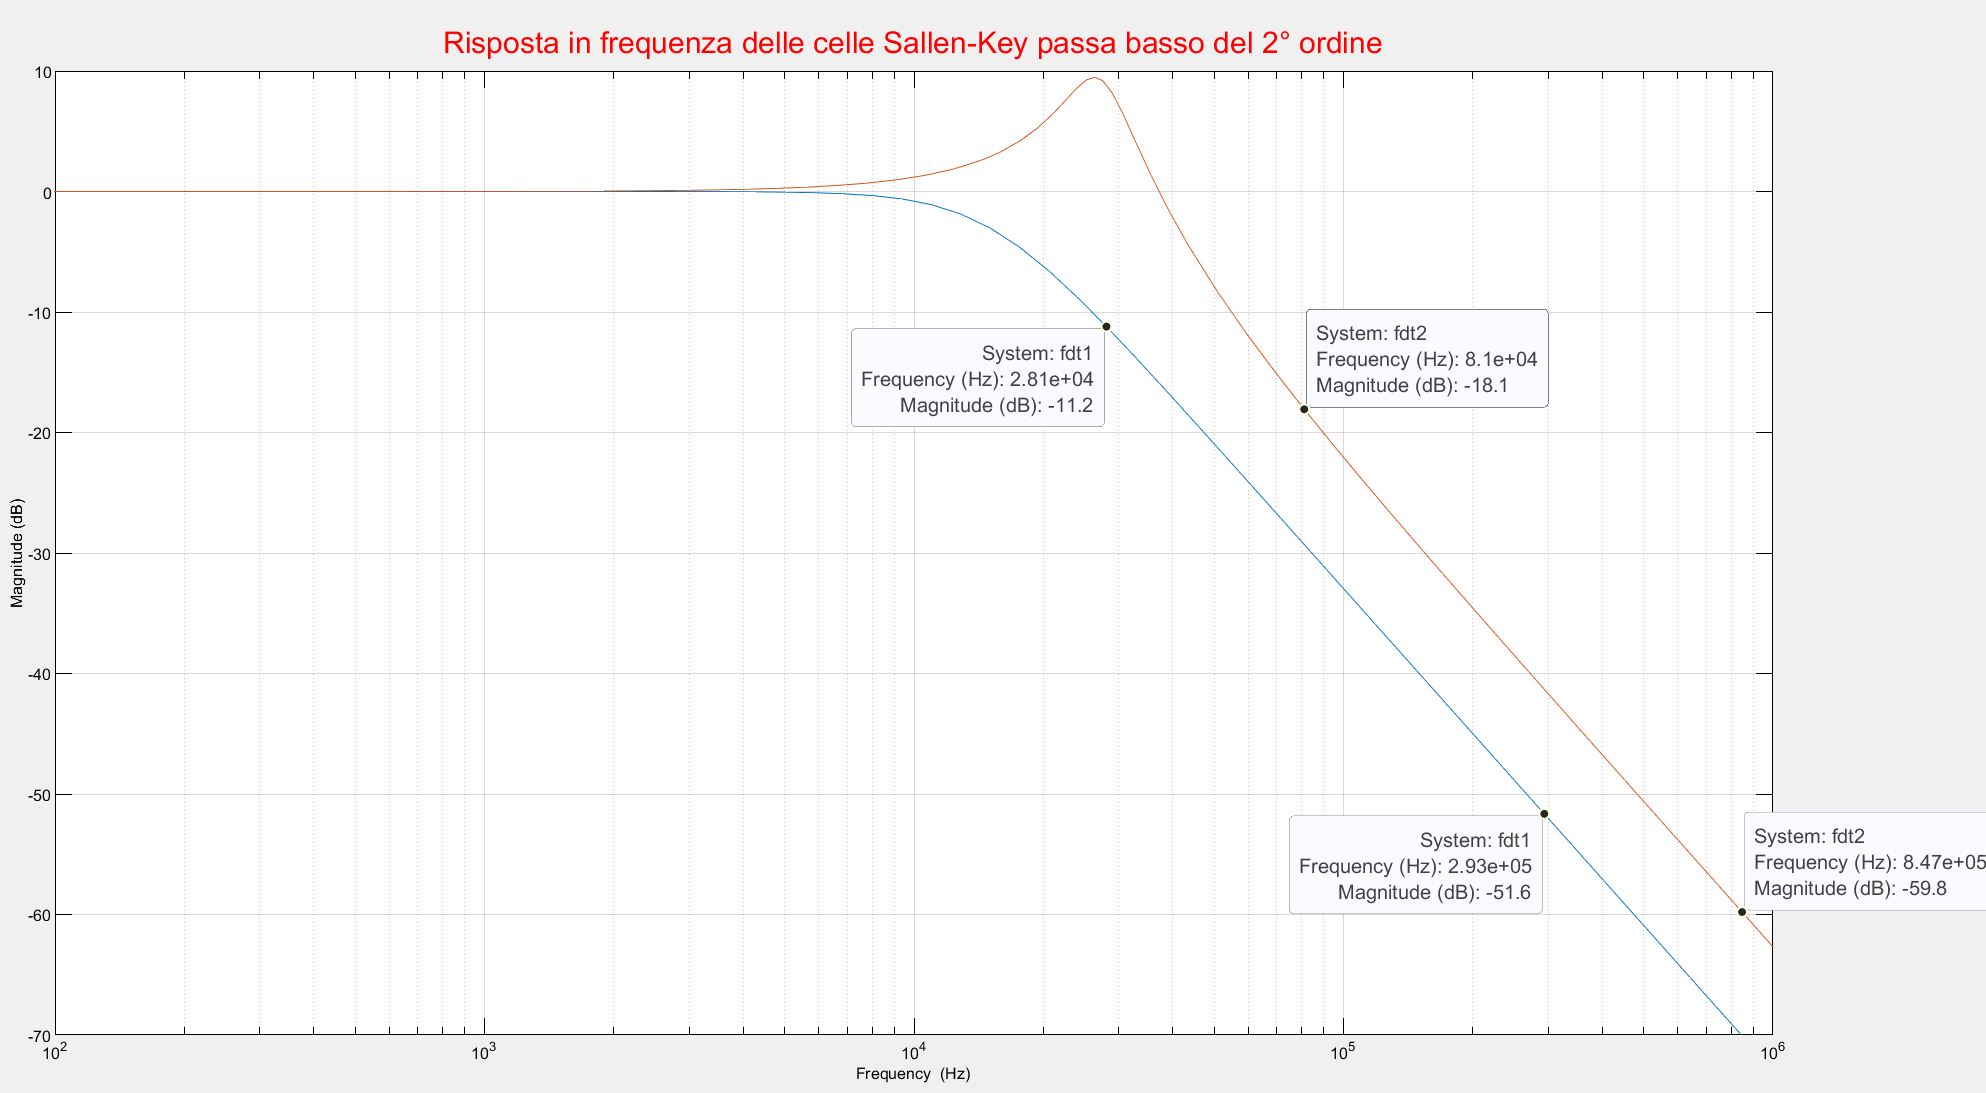
\includegraphics[scale=0.48]{Immagini/bode_lp2_tag.png}
		\caption{Diagramma di Bode delle celle Sallen-Key del $2^o$ ordine, che compongono il filtro del $4^o$ ordine}
		\label{fig:BODELp4Realzoom}
	\end{figure}
	

\newpage
\section{Filtro passa alto del primo ordine}
\label{sec:filtro_hp1}
	Per eliminare la componente in continua in uscita dal mixer analogico è necessario un filtro passa alto. L'elemento disaccoppiante più semplice da poter inserire è una capacità, tra uscita del mixer e l'uscita del sistema completo.
	Dovendo rispettare da specifiche una frequenza minima del segnale di uscita di \textit{20Hz} si è deciso di optare per la realizzazione di un filtro passa alto con frequenza di taglio di \textit{20Hz}. Tuttavia si è scelto di utilizzare un filtro attivo per recuperare l'attenuazione di fattore 10 imposta dall'\textit{AD633}, oltre che per disaccopiare il circuito dal carico.
	
	Da datasheet il prodotto banda guadagno (\textit{GBP}) dell'\textit{uA741} risulta essere di \textit{1MHz} in anello aperto. Tuttavia, utilizzando un guadagno di fattore 10 in anello chiuso, la banda passante del componente è ridotta a \textit{100kHz}. In questo modo è possibile ottenere un filtro passa banda con banda pari a \textit{20Hz - 100KHz}. Questo aiuta ad attenuare ulteriormente tutte le componenti in alta frequenza.
	Come mostra la \textit{Figura \ref{fig:gbp_ua741}}, l'ampiezza massima del segnale in uscita dal componente viene ridotta per le alte frequenze. Ciò implica che l'uscita finale del sistema oscillerà con un ampiezza massima di \textit{$\pm$6V}.

	\begin{figure}[H]
		\centering
		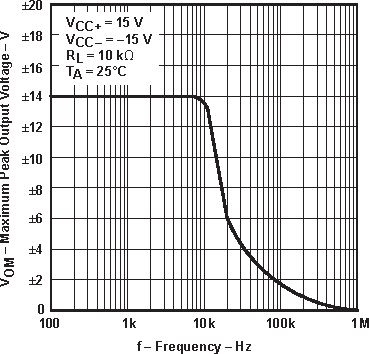
\includegraphics[scale=1]{Immagini/gbp_ua741.pdf}
		\caption{Ampiezza massima del segnale di uscita in relazione alla sua frequenza}
		\label{fig:gbp_ua741}
	\end{figure}

	Un'altro parametro importante da tenere in considerazione è il \textit{THD} che da datasheet risulta essere solo dello \textit{0.06\%} del segnale in ingresso. Quindi l'utilizzo di questo componente non introduce distorsione armonica significativa al sistema visti i valori esposti in precedenza.
	
	\begin{figure}[H]
		\centering
		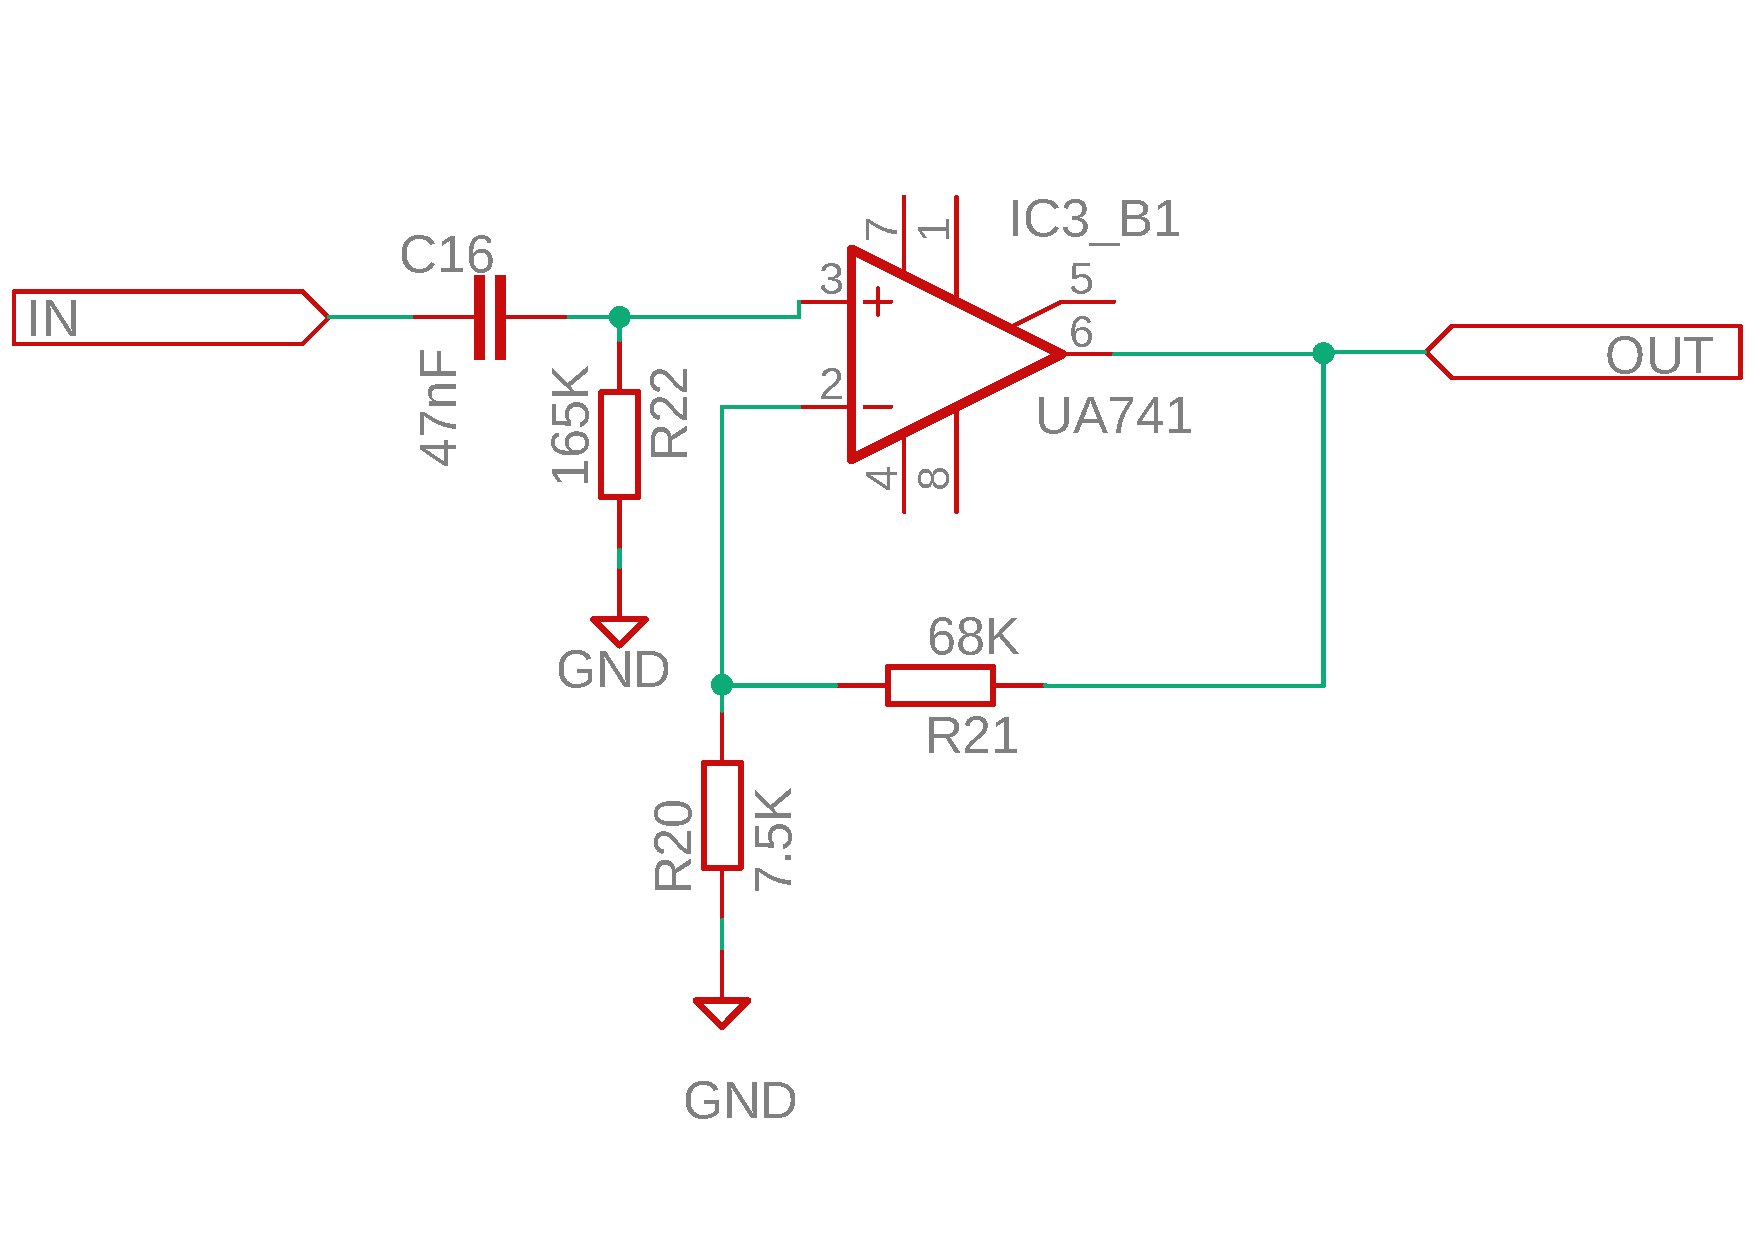
\includegraphics[scale=0.5]{Immagini/sch_hp1.pdf}
		\caption{Schema del filtro attivo passa alto del primo ordine}
		\label{fig:sch_hp1}
	\end{figure}

	In \textit{Figura \ref{fig:BODEHp1Real}} si può notare come il filtro teorico (mostrato in blu) e quello sperimentale (mostrato in rosso) abbiano un andamento simile, ma non siano sovrapposti. Il filtro sperimentale rispetta la specifica di progetto del limite inferiore di banda passante di \textit{20Hz}. Possiamo dire che il filtro attenua il segnale con frequenze inferiori a \textit{1Hz} in quanto si trova ad un valore di \textit{-20dB}. Per quanto riguarda le frequenze comprese tra \textit{1Hz e 20Hz} è vero dire che risultano amplificate, ma di un valore inferiore rispetto alla banda passante del filtro. Questo non risulta essere un problema poiché i due stadi precedenti, \textit{LP4} e il \textit{mixer}, attenuano il prodotto delle sinusoidi in ingresso al filtro di un valore 20. Pertanto le armoniche fuori dalla banda passante del filtro passa alto risultano comunque attenuate. Il risultato finale è riportato in \textit{Figura \ref{fig:FFTfinale}}.

	\begin{figure}[H]
		\centering
		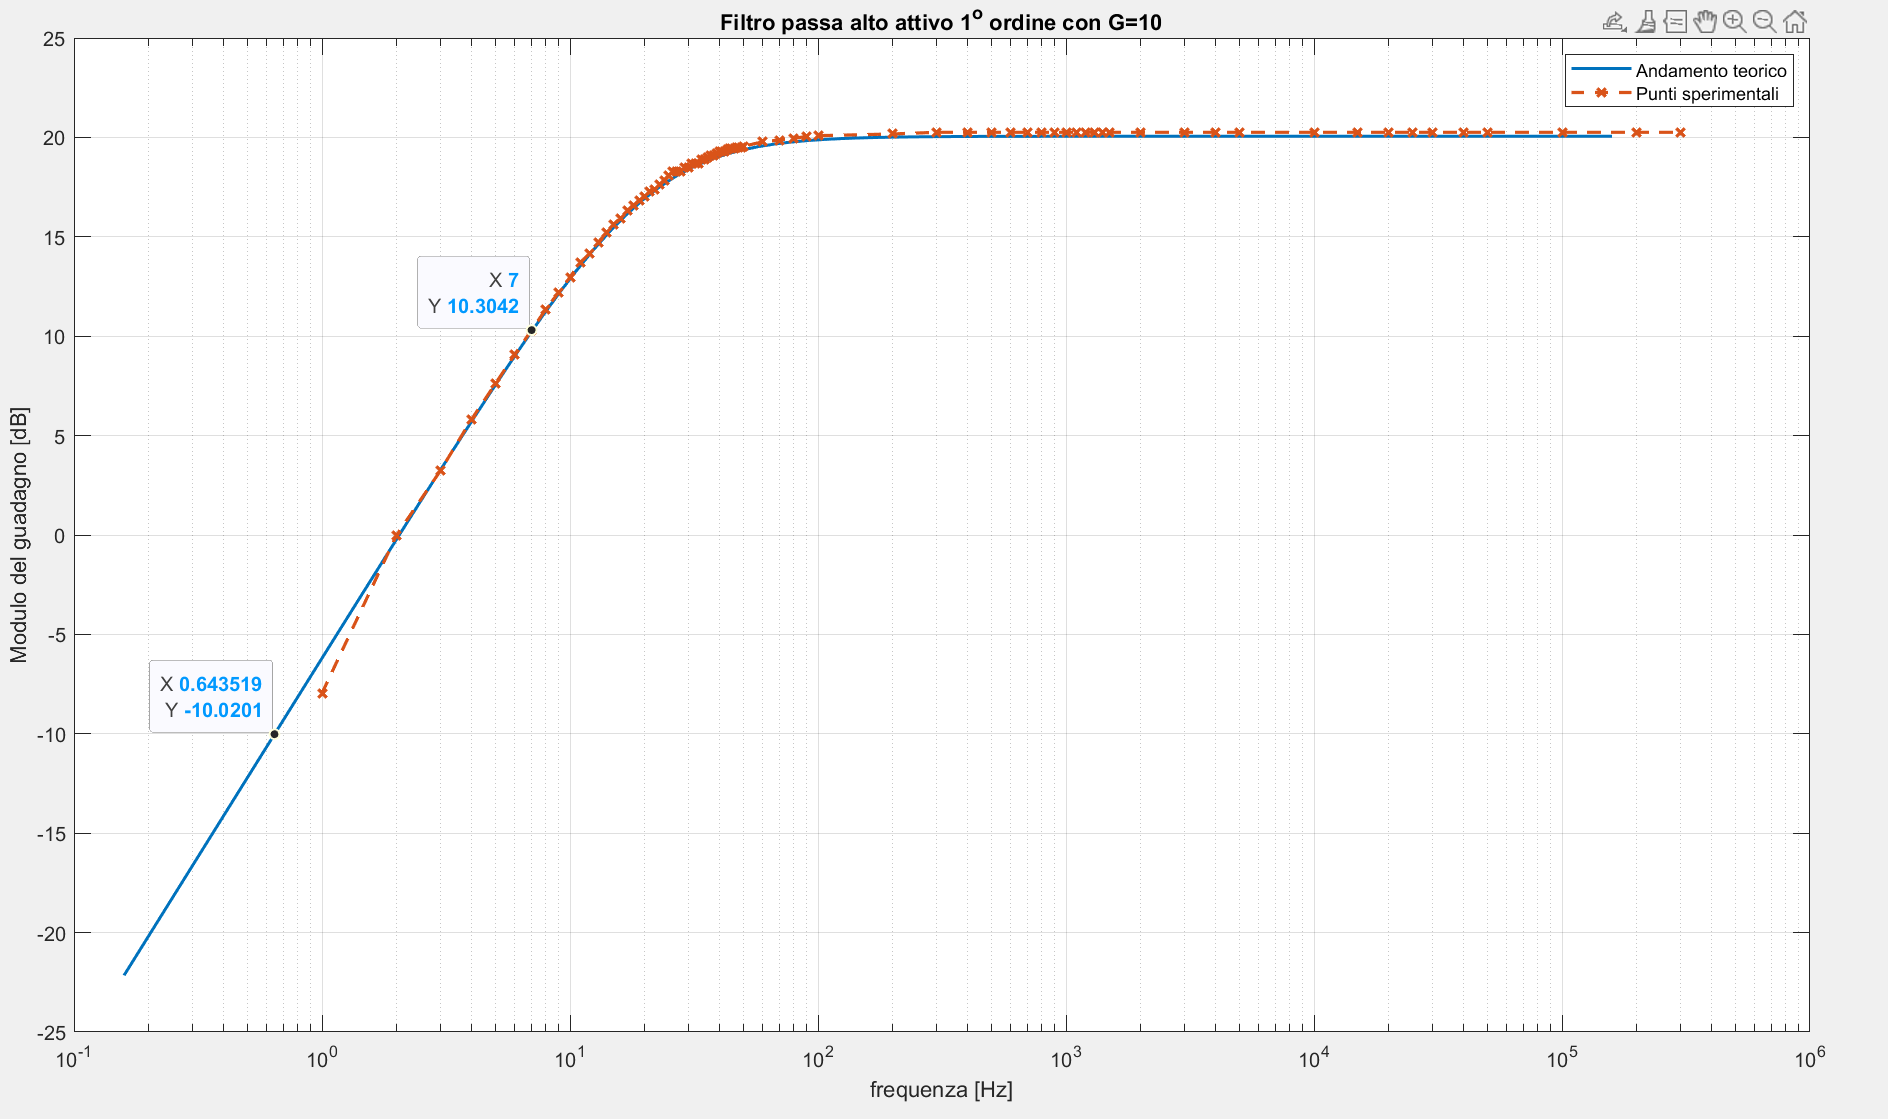
\includegraphics[scale=0.48]{Immagini/hpf1_filter_response.png}
		\caption{Diagramma di Bode del filtro passa alto del $1^o$ ordine}
		\label{fig:BODEHp1Real}
	\end{figure}


\newpage
\section{Theremin}
\label{ch:Teremin}

	In \textit{Figura \ref{fig:Schematico Completo}} è riportato lo schema circuitale completo del Theremin. Si possono osservare i vari blocchi introdotti nei capitoli precendenti e come vengono posti in relazione tra loro.

	\begin{figure}[H]
		\centering
		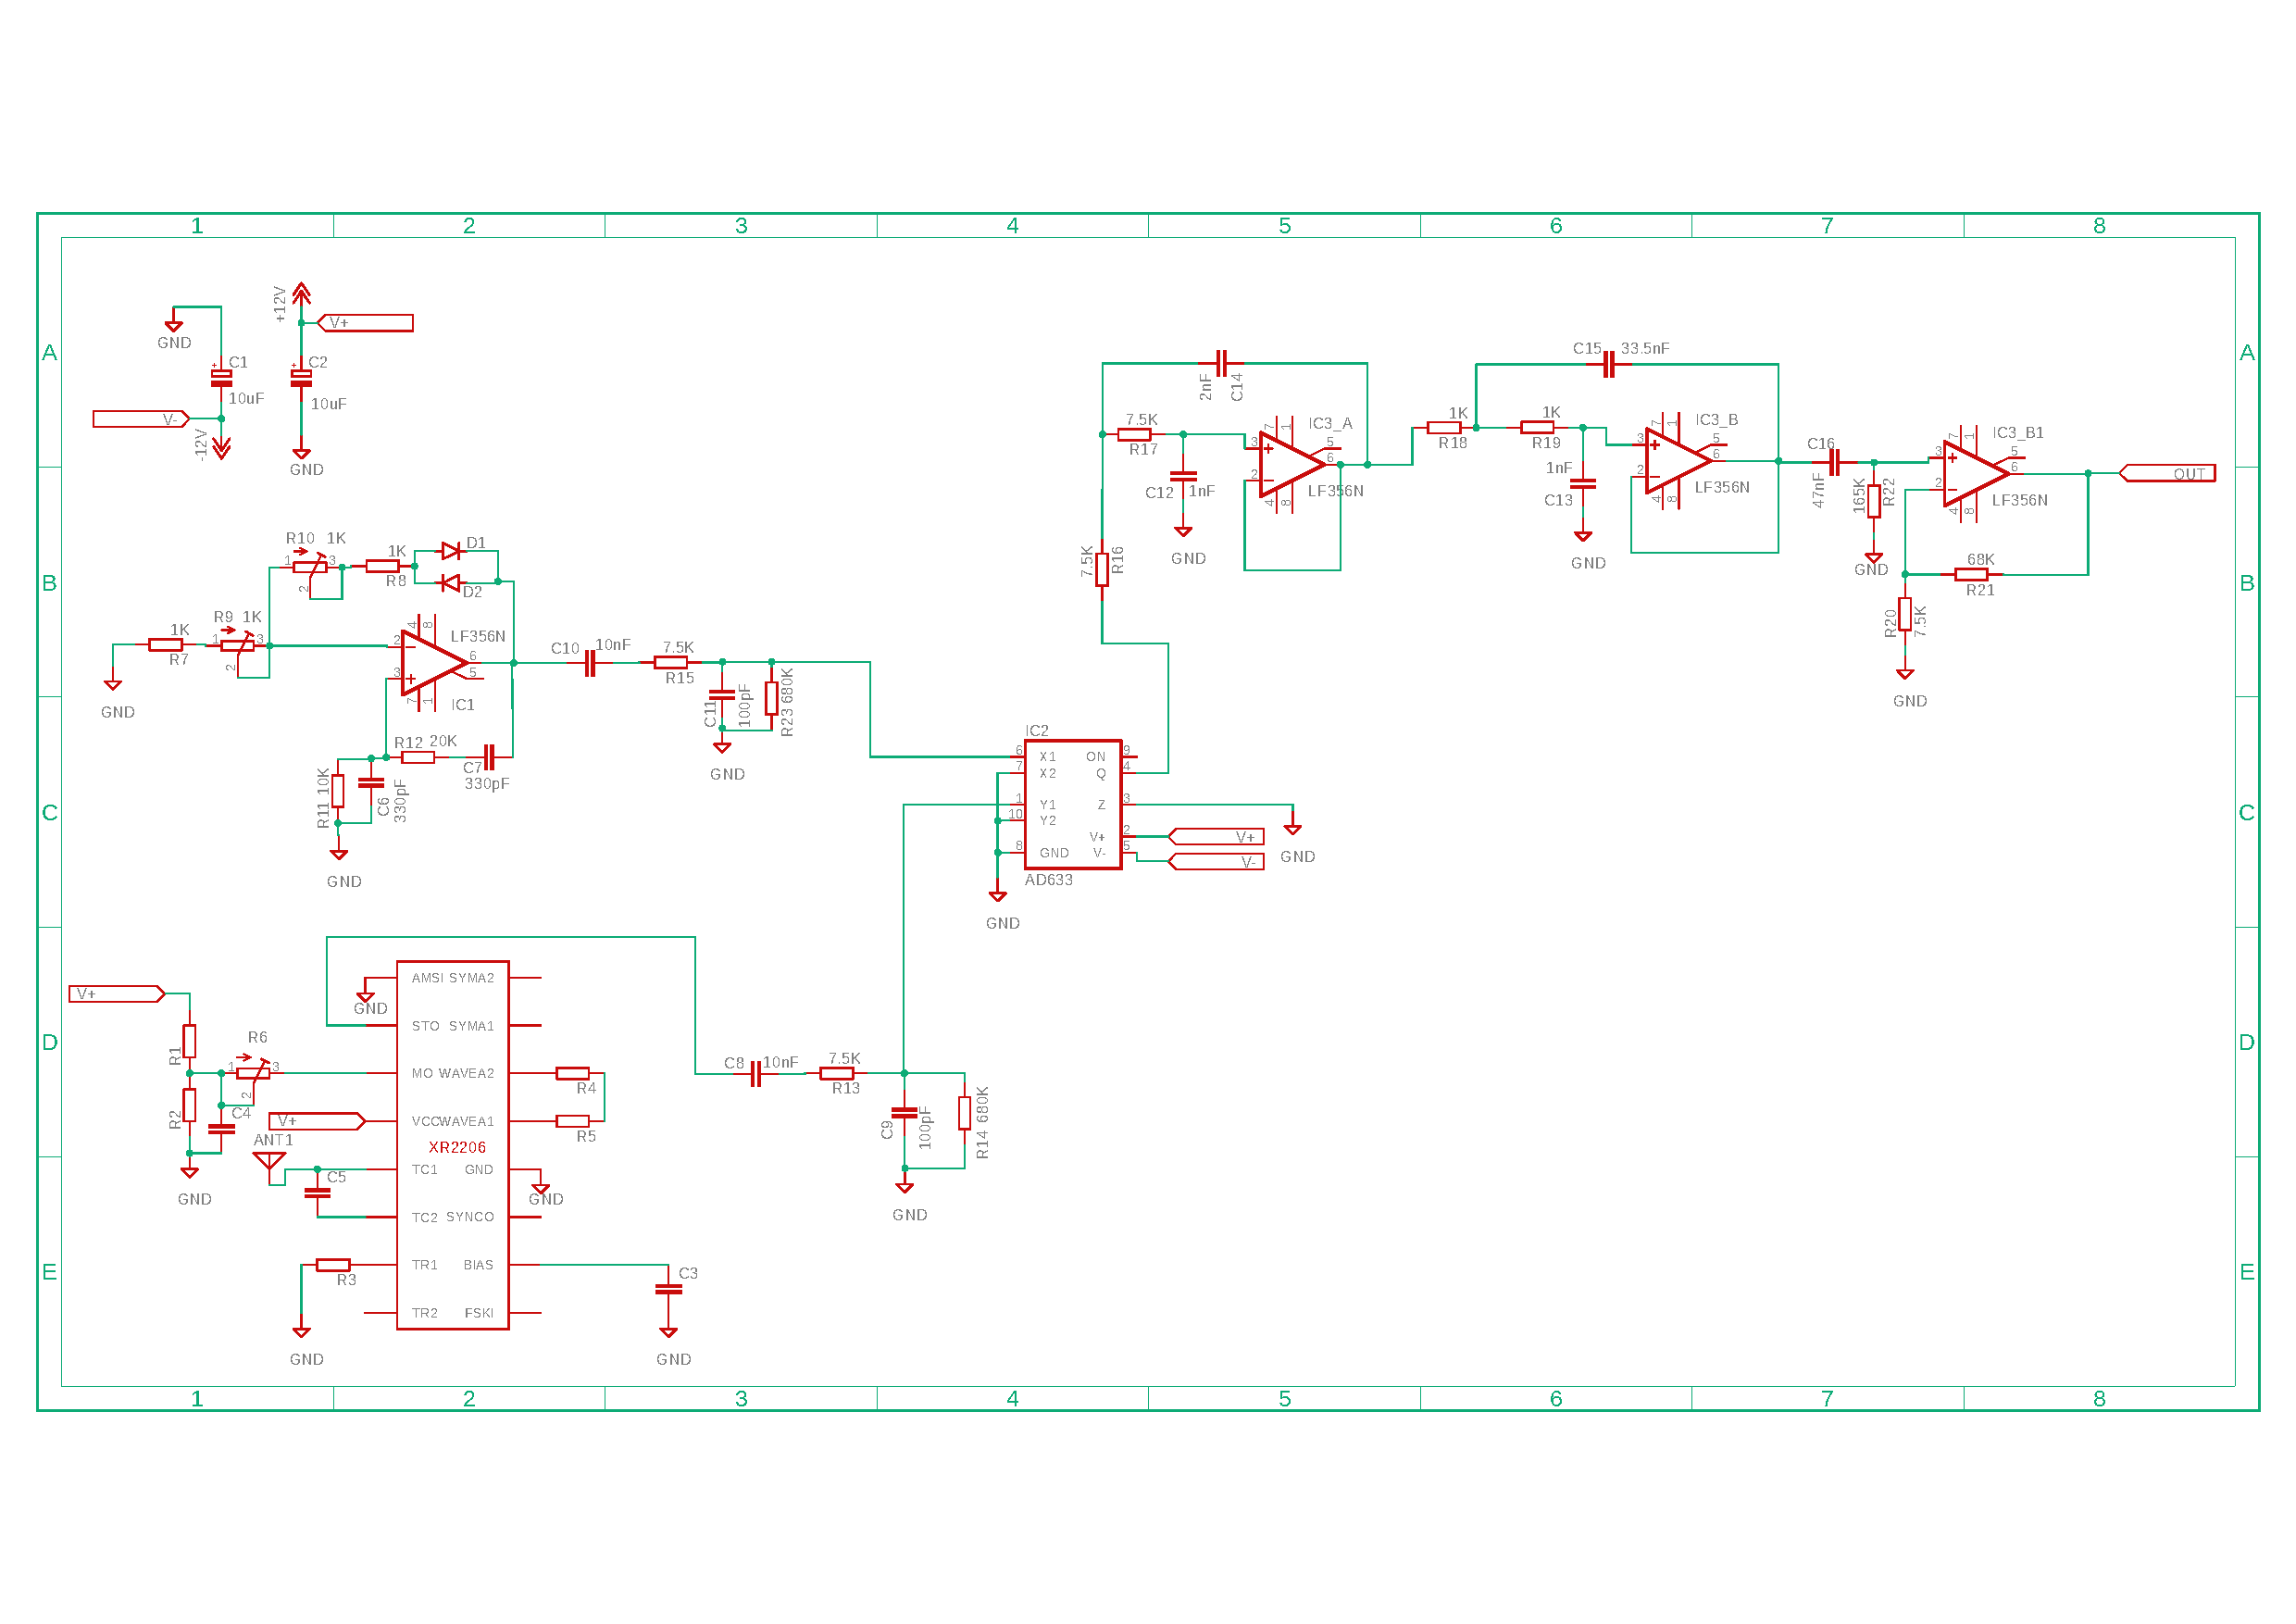
\includegraphics[scale=0.4]{Immagini/Schematico Completo.pdf}
		\caption{Schematico completo del circuito realizzato}
		\label{fig:Schematico Completo}
	\end{figure}

	\noindent La scelta delle frequenze operative nell'ordine del centinaio di \textit{kHz} è stata obbligata per poter avere una risoluzione accettabile in frequenza avvicinando la mano alla capacità variabile collegata al \textit{VCO}.
	Come si è visto nelle sezioni precedenti e come è riportato nella \textit{Figura \ref{fig:FFTwien+BP}} e in \textit{Figura \ref{fig:FFTxr+LP}}.

	\noindent Necessario è stato l'inserimento del filtro passa basso del quarto ordine in cascata al mixer. Questo ha portato ad un notevole miglioramento del \textit{THD} del segnale in uscita, come mostra la \textit{FFT} riportata in \textit{Figura \ref{fig:FFTAD33+LP4}}, nella quale si può notare la presenza di una singola armonica. L'oscilloscopio utilizzato non ha permesso di rilevare altre armoniche con la scala impostata, quindi non è stato possibile valutare il \textit{THD} del segnale.
	
	\begin{figure}[H]
		\centering
		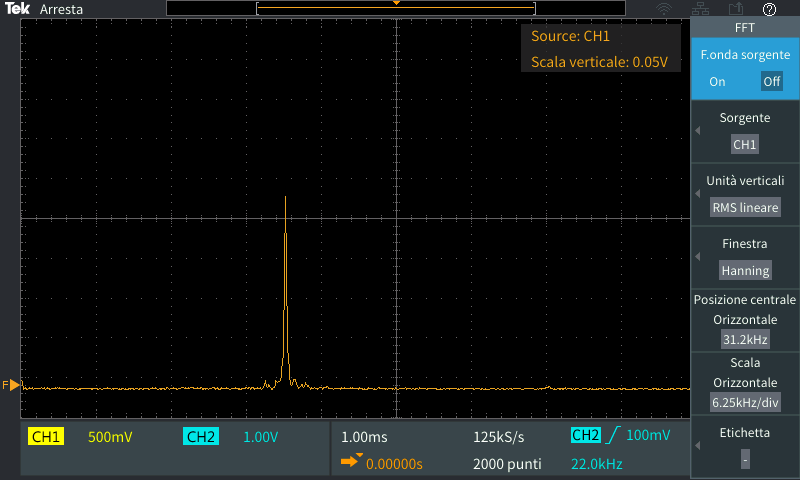
\includegraphics[scale = 0.5]{Immagini/fft_ad633+lp4.PNG}
		\caption{FFT in uscita dall'AD633 dopo il Filtro passa basso del quarto ordine}
		\label{fig:FFTAD33+LP4}
	\end{figure}

	L'aggiunta del filtro attivo passa alto è stato introdotto per tagliare la componente continua e le armoniche inferiori ai \textit{20Hz}.
	In \textit{Figura \ref{fig:FFTfinale}} è possibile osservare l'uscita complessiva del sistema.

	\begin{figure}[H]
		\centering
		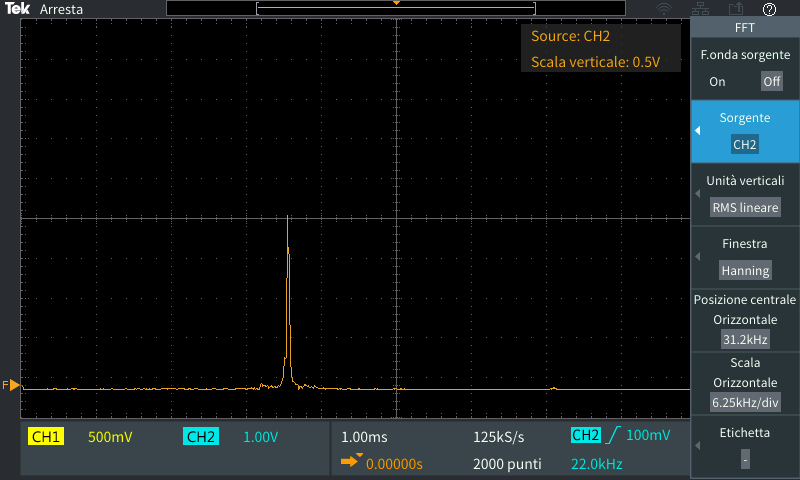
\includegraphics[scale = 0.5]{Immagini/ftt_ad633+lp4+hp1_final.PNG}
		\caption{FFT della sinusoide in uscita dal sistema}
		\label{fig:FFTfinale}
	\end{figure}

	È importante notare come in relazione alla \textit{Figura \ref{fig:FFTAD33+LP4}} l'introduzione del filtro passa alto non abbia portato un miglioramento apprezzabile al sistema. Tuttavia si può notare che la sinusioide in in uscita al filtro passa basso del quarto ordine, indicata in colore giallo, abbia delle componenti in alta frequenza evienziate dagli spikes che si vedono sovrapposti alla sinusoide principale. Tali spikes, vengono eliminati dallo stadio successivo, ovvero il passa alto attivo. Questo accade perchè il passa alto è stato realizzato utilizzando l'amplificatore operazione UA741. Questo tipo di operazionale ha un rapporto guadagno banda (\textit{GBP}) che cala la banda passante in relazione al guadagno impostato dall'amplificatore, come spiegato nella \textit{Sezione \ref{sec:OpAmp}}. Questo componente dunque agisce da filtro passa basso per costruzione. Uilizzandolo per realizzare un filtro passa alto attivo si ottiene un filtro passa banda, come somma dei due effetti, che va selezionare una banda passante di frequenze non attenuate.
	 
	 \begin{figure}[H]
		\centering
		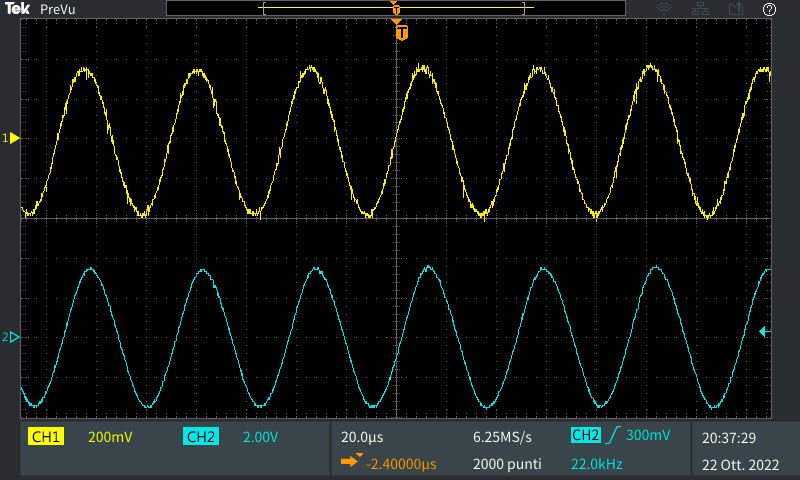
\includegraphics[scale = 0.5]{Immagini/sin_ad633+lp4_ad633+lp4+hp1.PNG}
		\caption{Sinusoidi in uscita dall'AD633 senza e con il filtro passa alto}
		\label{fig:AD33+LPconsenzaHP}
	\end{figure}


	La variazione di frequenza si manifesta con l'avvicinamento o l'allontanamento della mano dell'utente dalla bandiera, che compone l'altra faccia della capacità variabile. La variazione di capacità determinata dalla posizione della mano determina quindi la variazione di frequenza.
	In origine avevamo deciso di utilizzare una frequenza di riferimento di \textit{45kHz} per poi variare il segnale generato dal \textit{VCO} a frequenza che andassero da circa \textit{45kHz} a circa \textit{45kHz}.
	Tuttavia, è stato immediatamente riscontrato il problema della sensibilità, ovvero si è osservato come le uniche variazioni di frequenza apprezzabili si ottenessero quando la mano era posta a contatto con l'antenna o se quest'ultima fosse completamente assente. Si riusciva dunque a coprire una piccolissima parte del range richiesto dal progetto senza però ottenere le variazioni volute.
	Perciò, si è deciso di alzare le frequenze operative, portando il riferimento in uscita dall'oscillatore di Wien ad un valore di \textit{245kHz} come mostrato in \textit{Figura \ref{fig:SINwien+BP}}. Questo ha porta a dover aumentare anche il range di frequenze del \textit{VCO} portando così gli estremi da un'oscillazione di \textit{275kHz} senza la presenza della mano a circa \textit{250kHz} con la presenza della mano ad una distanza minima ove la mano risultasse quasi a contatto con l'antenna.
	In questo caso, si è riscontrato un netto miglioramento della sensibilità nella variazione della frequenza rispetto alla distanza della mano.
	Nella \textit{Tabella \ref{tab:Distanza-Frequenza}} sono mostrati i risultati sperimentali ottenuti misurando la frequenza di oscillazione del segnale di uscita in relazione alla distanza della mano dalla bandiera. \newline	
%\section{Problematiche}

% Cosa succede se la distorsione è sull'amplificatore, piuttosto che sull'oscillatore piuttosto che sull'XR? Bisogna che i componenti siano a bassa distorsione armonica.
	
	% Se il segnale in uscita all'oscillatore di wien fosse triangolare, cosa accade dopo il motiplicatore? Prossima lezione si vedrà cosa accade se il segnale è un onda quadra.


	% L'xr2206 inserisce un offset grazie al quale riesce a far oscillare l'uscita, il ptenziomentro R3 serve a gestire tale oscillazione mandando in saturazione o meno, mentre R5 aggiusta le componenti armoniche.

	%\label{FIGURE}
	
	\begin{table}[h!]
		\centering
		\begin{tabular}{||c|c|c||}
			\hline
			\cellcolor{gray!10}Distanza [cm] & \cellcolor{gray!10}Frequenza [kHz] \\
			\hline
			15 & 272 \\
			\hline
			14 & 272 \\
			\hline
			13 & 273 \\
			\hline
			12 & 273 \\
			\hline
			11 & 272 \\
			\hline
			10 & 272 \\
			\hline		
			9 &  272 \\
			\hline
			8 &  271 \\
			\hline
			7 &  269 \\
			\hline
		    6 &  270 \\
			\hline
			5 &  267 \\
			\hline
			4 &  265 \\
			\hline
			3 &  260 \\
			\hline
			2 &  259 \\
			\hline
			1 &  249 \\
			\hline
			0 &  244 \\
			\hline
		\end{tabular}
		\caption{Relazione distanza della mano dell'utente dall'antenna - frequenza di oscillazione della sinusoide prodotta}
		\label{tab:Distanza-Frequenza}
	\end{table}
	
	Dalla tabella \ref{tab:Distanza-Frequenza} si è calcolato la sensibilità relativa del sistema completo al variare della distanza della mano dall'antenna. \newline
	In figura \ref{fig:sens_sistema} vengono mostrati i punti ottenuti sperimentalmente e una curva ottenuta con un'approssimazione ai minimi quadrati utilizzando un polinomio di grado 3. Dalla figura è possibile osservare come la sensibilità sia molto elevata per distanze mano-antenna molto piccole, mentre sia pressoché nulla quando la mano supera gli 8 cm di distanza dall'antenna.
	\begin{figure}[H]
		\centering
		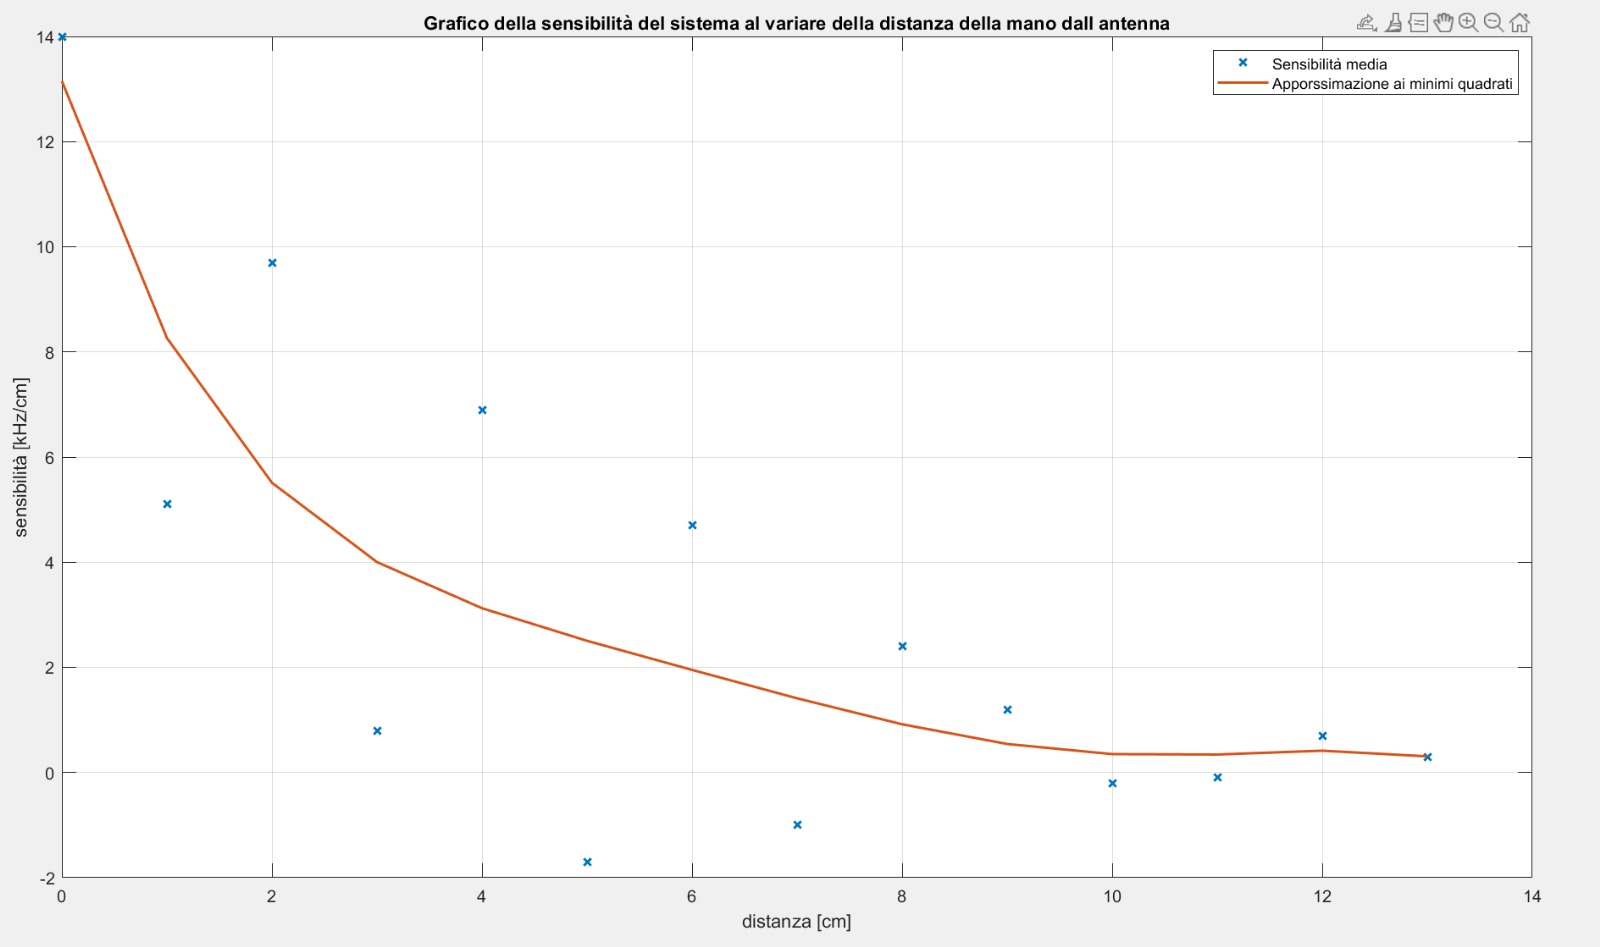
\includegraphics[scale = 0.4]{Immagini/sens_poly.jpg}
		\caption{Sensibilità del sistema}
		\label{fig:sens_sistema}
	\end{figure}
%\newpage
%	\begin{figure}[]
%		\centering
%		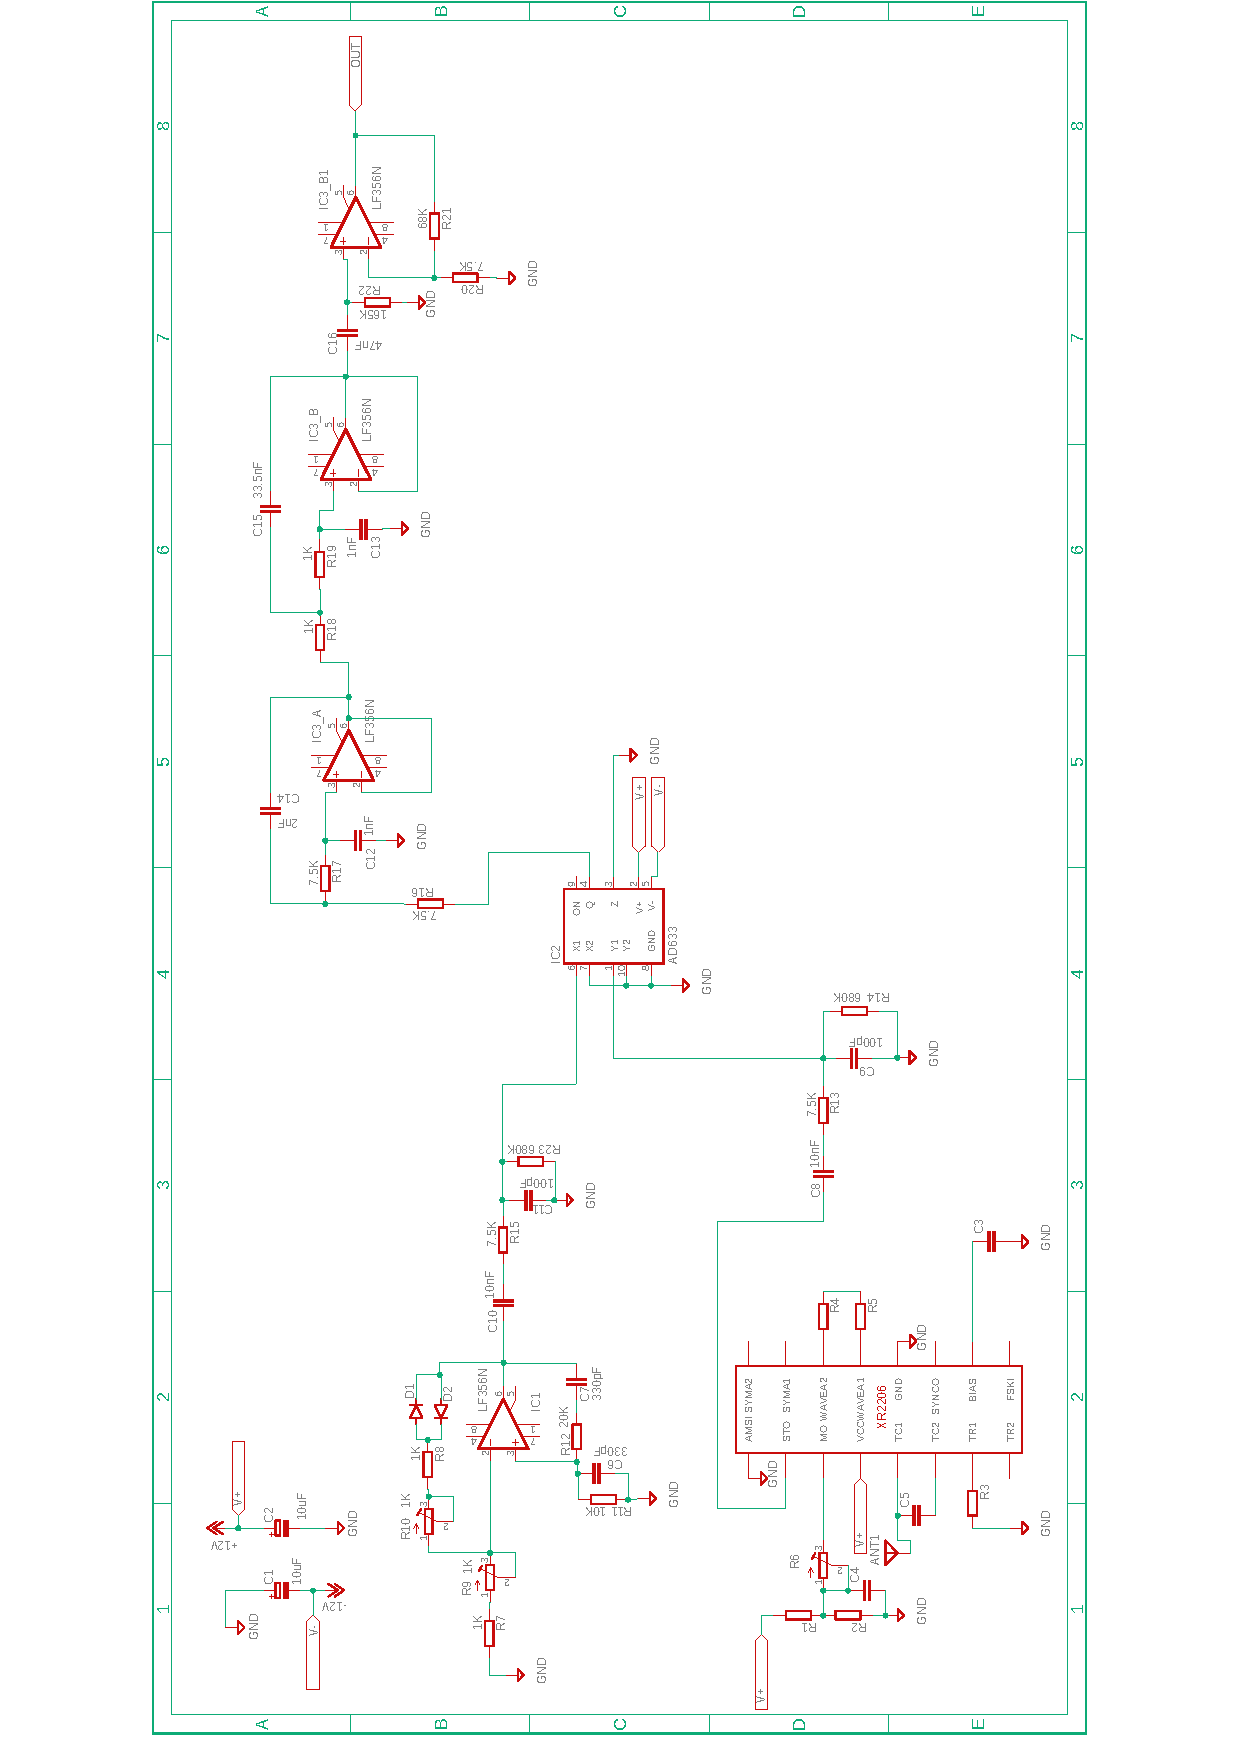
\includegraphics[scale=0.8]{Immagini/sch_complet_a4_verticale.pdf}
%		\caption{Schematico completo del circuito realizzato}
%		\label{fig:sch_completo_verticale}
%	\end{figure}

\chapter{Conclusioni}
 	\label{ch:Conclusioni}

	In conclusione, il circuito realizzato rispetta le specifiche di progetto, in quanto testando con un generatore di funzione i filtri, in uscita essi garantiscono il passaggio di sinusoidi con frequenza compresa tra \textit{20Hz e 20kHz}. Osservando la \textit{Tabella \ref{tab:Distanza-Frequenza}} si può osservare che i limiti inferiore e superiore concordano con la scelta di un oscillazione di \textit{245kHz} per l'oscillatore di Wien. Infatti, l'uscita complessiva del sistema oscilla tra \textit{22kHz} in assenza della mano, fino a \textit{1kHz} quando la mano è in prossimità dell'antenna. Il risultato non è ottimo ma abbastanza soddisfacente visti i limiti fisici dovuti agli strumenti a disposizione. Infatti, il limite inferiore di oscillazione del sistema è dovuto soltato ai disturbi generati dall'antenna quando la mano è molto vicina (circa 2cm di distanza). Le frequenze nell'ordine delle centinaia di \textit{kHz} permettono di avere delle variazioni apprezzabili sulla frequenza in uscita al sistema. Ovvero la riduzione della frequenza della sinusoide risulta proporzionale alla distanza della mano dall'antenna.
	Non sono stati imposti vincoli sulla risoluzione, principale tallone d'Achille del sistema realizzato. La risoluzione infatti non risulta costante, inoltre man mano ci si avvicina con la mano all'antenna il sistema risulta meno sensibile. Infatti, non è possibile rilevare variazioni inferiori al \textit{kHz}.
	Il problema della risoluzione potrebbe essere risolto migliorando il sistema utilizzato per la realizzazione della capacità variabile. Inoltre, aumentando la frequenza di oscillazione dell'\textit{XR2206} è possibile ottenere una sensibilità maggiore poiché per aumentare la frequenza di oscillazione è necessario utilizzare capacità molto piccole (dell'ordine del pF) confrontabili con la capacità formata tra antenna e mano. Questo fa in modo di attuare una variazione di capacità molto incisiva per la generazione del segnale, il quale avrà una risoluzione maggiore.
	\newpage
	

	\section{MODIFICHE}
	Risistemare il ponte di wien, rifare le immagini dello spetro e del THD
	Sistemare il grafico dei filtri \newline
	\noindent
	studio e progetto dei filtri passa banda passivi
	\noindent
	come funziona il VCO dell/XR e il sine shaper
	\newline
	FFT del mixer da rifare \newline
	Sch ponte di wien e calcolo in V del THD della sinusoide di uscita
	\listoffigures
	\listoftables
\end{document}
